%%%%%%%%%%%%%%%%%%%%%%%%%%%%%%%%%%%%%%%%%
% Masters/Doctoral Thesis 
% LaTeX Template
% Version 2.1 (2/9/15)
%
% This template has been downloaded from:
% http://www.LaTeXTemplates.com
%
% Version 2.0 major modifications by:
% Vel (vel@latextemplates.com)
%
% Original authors:
% Steven Gunn  (http://users.ecs.soton.ac.uk/srg/softwaretools/document/templates/)
% Sunil Patel (http://www.sunilpatel.co.uk/thesis-template/)
%
% License:
% CC BY-NC-SA 3.0 (http://creativecommons.org/licenses/by-nc-sa/3.0/)
%
%%%%%%%%%%%%%%%%%%%%%%%%%%%%%%%%%%%%%%%%%

%----------------------------------------------------------------------------------------
%	PACKAGES AND OTHER DOCUMENT CONFIGURATIONS
%----------------------------------------------------------------------------------------

\documentclass[
11pt, % The default document font size, options: 10pt, 11pt, 12pt
%oneside, % Two side (alternating margins) for binding by default, uncomment to switch to one side
english, % ngerman for German
singlespacing, % Single line spacing, alternatives: onehalfspacing or doublespacing
%draft, % Uncomment to enable draft mode (no pictures, no links, overfull hboxes indicated)
%nolistspacing, % If the document is onehalfspacing or doublespacing, uncomment this to set spacing in lists to single
%liststotoc, % Uncomment to add the list of figures/tables/etc to the table of contents
%toctotoc, % Uncomment to add the main table of contents to the table of contents
%parskip, % Uncomment to add space between paragraphs
]{MastersDoctoralThesis} % The class file specifying the document structure

\usepackage[utf8]{inputenc} % Required for inputting international characters
\usepackage[T1]{fontenc} % Output font encoding for international characters

\usepackage{palatino} % Use the Palatino font by default

\usepackage[backend=bibtex,style=authoryear,natbib=true]{biblatex} % User the bibtex backend with the authoryear citation style (which resembles APA)

\addbibresource{example.bib} % The filename of the bibliography

\usepackage[autostyle=true]{csquotes} % Required to generate language-dependent quotes in the bibliography

\usepackage{amssymb,amsmath}
\usepackage{amsfonts}

%----------------------------------------------------------------------------------------
%	INCLUDE DEFINITIONS FILE
%----------------------------------------------------------------------------------------
%----------------------------------------------------------------------------------------
%	DEFINE CUSTOM SYMBOL COMMANDS
%----------------------------------------------------------------------------------------

% Bold
\def\u{{\bf u}}
\def\x{{\bf x}}
\def\r{{\bf r}}
\def\e{{\bf e}}
\def\a{{\bf a}}
\def\v{{\bf v}}
\def\w{{\bf w}}
\def\f{{\bf f}}
\def\n{{\bf n}}
\def\t{{\bf t}}
\def\k{{\bf k}}
\def\R{{\bf R}}
\def\F{{\bf F}}
\def\U{{\bf U}}
\def\P{{\bf P}}
\def\X{{\bf X}}
\def\H{\bf{H}}
\def\Lbf{{\bf L}}
\def\Hbf{{\bf H}}
\def\Tbf{{\bf T}}
\def\Cbf{{\bf C}}
\def\Rbf{{\bf R}}
\def\boldI{\mathbf{I}}

% Bold symbols
\def\XI{{\boldsymbol{\Xi}}}
\def\kppa{\boldsymbol{\kappa}}
\def\etaa{\boldsymbol{\eta}}
\def\xii{\boldsymbol{\xi}}
\def\KA{\boldsymbol{\Kappa}}
\def\ETA{\boldsymbol{\Upsilon}}
\def\boldsigma{\boldsymbol{\sigma}}
\def\boldomega{\boldsymbol{\omega}}
\def\boldzeta{\boldsymbol{\zeta}}

%Caligraphic
\def\Dcal{\mathcal{D}}
\def\Ccal{\mathcal{C}}

% BB
\def\M{\mathbb{M}}
\def\K{\mathbb{K}}
\def\C{\mathbb{C}}
\def\G{\mathbb{G}}
\def\D{\mathbb{D}}
\def\L{\mathbb{L}}
\def\A{\mathbb{A}}
\def\B{\mathbb{B}}
\def\I{\mathbb{I}}
\def\Sb{\mathbb{S}}
\def\Kt{\tilde{\mathbb{K}}}
\def\Bt{\tilde{\mathbb{B}}}
\def\Mt{\tilde{\mathbb{M}}}
\def\St{\tilde{\mathbb{S}}}
\def\At{\tilde{\mathbb{A}}}
\def\T{\mathbb{T}}
\def\Rbb{\mathbb{R}}

% Other
\def\half{\frac{1}{2}}
\def\Eq#1{(\ref{eq-#1})}
\def\Lem#1{\ref{lem-#1}}
\def\Fig#1{Figure \ref{fig-#1}}
\def\Chap#1{Chapter \ref{chap-#1}}
\def\Sec#1{Section \ref{sec-#1}}
\def\cl{ \nonumber \\}
\def\el{\nonumber}
\def\jumpl{\lbrack\!\lbrack}
\def\jumpr{\rbrack\!\rbrack}
\def\jump#1{\jumpl #1 \jumpr}
\def\jumpt#1{\underline{\jump{#1}}}
\def\mean#1{\{\! \!\{ #1\}\! \!\}}
\def\meanpv#1{\{ #1\}}
\def\meanhar#1{\langle#1\rangle}
\def\Qq{ \Omega \times (0,t^*)}

% New commands
\newtheorem{remark}{Remark}[section]
\newtheorem{proposition}{Proposition}[section]
\newcommand{\tickYes}{\checkmark}
\newcommand{\tickNo}{\hspace{1pt}\ding{55}}
\definecolor{tableShade}{HTML}{F1F5FA}



%----------------------------------------------------------------------------------------
%	THESIS INFORMATION
%----------------------------------------------------------------------------------------

\thesistitle{Thesis Title} % Your thesis title, this is used in the title and abstract, print it elsewhere with \ttitle
\supervisor{Dr. Santiago \textsc{Badia}} % Your supervisor's name, this is used in the title page, print it elsewhere with \supname
\examiner{} % Your examiner's name, this is not currently used anywhere in the template, print it elsewhere with \examname
\degree{Doctor of Philosophy} % Your degree name, this is used in the title page and abstract, print it elsewhere with \degreename
\author{Oriol \textsc{Colomés}} % Your name, this is used in the title page and abstract, print it elsewhere with \authorname
\addresses{} % Your address, this is not currently used anywhere in the template, print it elsewhere with \addressname

\subject{} % Your subject area, this is not currently used anywhere in the template, print it elsewhere with \subjectname
\keywords{} % Keywords for your thesis, this is not currently used anywhere in the template, print it elsewhere with \keywordnames
\university{\href{http://www.upc.edu}{Universitat Politècnica de Catalunya}} % Your university's name and URL, this is used in the title page and abstract, print it elsewhere with \univname
\department{\href{http://www.cimne.com}{Centre Internacional de Mètodes Numèrics en Enginyeria}} % Your department's name and URL, this is used in the title page and abstract, print it elsewhere with \deptname
\group{\href{http://www.cimne.com/spacehome/2/1156}{Large Scale Scientific Computing group}} % Your research group's name and URL, this is used in the title page, print it elsewhere with \groupname
\faculty{\href{http://www.camins.upc.edu}{Escola Tècnica Superior d'Enginyeria de Camins, Canals i Ports de Barcelona}} % Your faculty's name and URL, this is used in the title page and abstract, print it elsewhere with \facname

\hypersetup{pdftitle=\ttitle} % Set the PDF's title to your title
\hypersetup{pdfauthor=\authorname} % Set the PDF's author to your name
\hypersetup{pdfkeywords=\keywordnames} % Set the PDF's keywords to your keywords

\begin{document}

\frontmatter % Use roman page numbering style (i, ii, iii, iv...) for the pre-content pages

\pagestyle{plain} % Default to the plain heading style until the thesis style is called for the body content

%----------------------------------------------------------------------------------------
%	TITLE PAGE
%----------------------------------------------------------------------------------------

\begin{titlepage}
\begin{center}

\textsc{\LARGE \univname}\\[1.5cm] % University name
\textsc{\Large Doctoral Thesis}\\[0.5cm] % Thesis type

\HRule \\[0.4cm] % Horizontal line
{\huge \bfseries \ttitle}\\[0.4cm] % Thesis title
\HRule \\[1.5cm] % Horizontal line
 
\begin{minipage}{0.4\textwidth}
\begin{flushleft} \large
\emph{Author:}\\
%\href{http://www.johnsmith.com}{\authorname} % Author name - remove the \href bracket to remove the link
{\authorname} % Author name - remove the \href bracket to remove the link
\end{flushleft}
\end{minipage}
\begin{minipage}{0.4\textwidth}
\begin{flushright} \large
\emph{Supervisor:} \\
%\href{http://www.jamessmith.com}{\supname} % Supervisor name - remove the \href bracket to remove the link  
{\supname} % Supervisor name - remove the \href bracket to remove the link  
\end{flushright}
\end{minipage}\\[3cm]
 
%\large \textit{A thesis submitted in fulfilment of the requirements\\ for the degree of \degreename}\\[0.3cm] % University requirement text
\large \textit{\degreename}\\[0.3cm] % University requirement text
\textit{in the}\\[0.4cm]
\groupname\\\deptname\\[2cm] % Research group name and department name
 
{\large \today}\\[4cm] % Date
%\includegraphics{Logo} % University/department logo - uncomment to place it
 
\vfill
\end{center}
\end{titlepage}

%----------------------------------------------------------------------------------------
%	DECLARATION PAGE
%----------------------------------------------------------------------------------------

\begin{declaration}
\addchaptertocentry{\authorshipname}

\noindent I, \authorname, declare that this thesis titled, \enquote{\ttitle} and the work presented in it are my own. I confirm that:

\begin{itemize} 
\item This work was done wholly or mainly while in candidature for a research degree at this University.
\item Where any part of this thesis has previously been submitted for a degree or any other qualification at this University or any other institution, this has been clearly stated.
\item Where I have consulted the published work of others, this is always clearly attributed.
\item Where I have quoted from the work of others, the source is always given. With the exception of such quotations, this thesis is entirely my own work.
\item I have acknowledged all main sources of help.
\item Where the thesis is based on work done by myself jointly with others, I have made clear exactly what was done by others and what I have contributed myself.\\
\end{itemize}
 
\noindent Signed:\\
\rule[0.5em]{25em}{0.5pt} % This prints a line for the signature
 
\noindent Date:\\
\rule[0.5em]{25em}{0.5pt} % This prints a line to write the date
\end{declaration}

\cleardoublepage

%----------------------------------------------------------------------------------------
%	QUOTATION PAGE
%----------------------------------------------------------------------------------------

\vspace*{0.2\textheight}

\noindent\enquote{\itshape Thanks to my solid academic training, today I can write hundreds of words on virtually any topic without possessing a shred of information, which is how I got a good job in journalism.}\bigbreak

\hfill Dave Barry

%----------------------------------------------------------------------------------------
%	ABSTRACT PAGE
%----------------------------------------------------------------------------------------

\begin{abstract}
\addchaptertocentry{\abstractname} % Add the abstract to the table of contents

The Thesis Abstract is written here (and usually kept to just this page). The page is kept centered vertically so can expand into the blank space above the title too\ldots

\end{abstract}

%----------------------------------------------------------------------------------------
%	ACKNOWLEDGEMENTS
%----------------------------------------------------------------------------------------

\begin{acknowledgements}
\addchaptertocentry{\acknowledgementname} % Add the acknowledgements to the table of contents

The acknowledgements and the people to thank go here, don't forget to include your project advisor\ldots

\end{acknowledgements}

%----------------------------------------------------------------------------------------
%	LIST OF CONTENTS/FIGURES/TABLES PAGES
%----------------------------------------------------------------------------------------

\tableofcontents % Prints the main table of contents

\listoffigures % Prints the list of figures

\listoftables % Prints the list of tables

%----------------------------------------------------------------------------------------
%	ABBREVIATIONS
%----------------------------------------------------------------------------------------

\begin{abbreviations}%{ll} % Include a list of abbreviations (a table of two columns)

%\textbf{LAH} & \textbf{L}ist \textbf{A}bbreviations \textbf{H}ere\\
%\textbf{WSF} & \textbf{W}hat (it) \textbf{S}tands \textbf{F}or\\
\textbf{DFFT} & \textbf{D}iscrete \textbf{F}ast \textbf{F}ourier \textbf{T}ransform \\
\textbf{SGS} & \textbf{S}ub\textbf{G}rid \textbf{S}cale\\
\textbf{RMS} & \textbf{R}oot \textbf{M}ean \textbf{S}quare\\

\end{abbreviations}

%----------------------------------------------------------------------------------------
%	PHYSICAL CONSTANTS/OTHER DEFINITIONS
%----------------------------------------------------------------------------------------

\begin{constants}%{lr@{${}={}$}l} % The list of physical constants is a three column table

 %The \SI{}{} command is provided by the siunitx package, see its documentation for instructions on how to use it

Speed of Light & $c$ & \SI{2.99792458e8}{\meter\per\second} (exact)\\
%Constant Name & $Symbol$ & $Constant Value$ with units\\

\end{constants}

%----------------------------------------------------------------------------------------
%	SYMBOLS
%----------------------------------------------------------------------------------------

%\begin{symbols}%{lll} % Include a list of Symbols (a three column table)
\begin{symbols}

$\u(\x,t)$ & velocity field       & \si{\meter\per\second} \\
$u_x$      & velocity x-component & \si{\meter\per\second} \\
$u_y$      & velocity y-component & \si{\meter\per\second} \\
$u_z$      & velocity z-component & \si{\meter\per\second} \\
$u$        & velocity RMS & \\
$\overline{\u}$ & time-averaged velocity component & \si{\meter\per\second} \\
$\u'$           & fluctuating velocity component   & \si{\meter\per\second} \\
$\hat{p}$       & pressure field                   & \si{\pascal}\\
$p(x,t)$        & kinematic pressure field                   & \si{\pascal}\\  
$\overline{p}$  & time-averaged pressure component & \si{\pascal}\\  
$p'$            & fluctuating pressure component   & \si{\pascal}\\  
$\f$            & External body force              & \si{\newton}\\
$\n$            & unit outward normal vector       &       \\
$l$             & integral length scale            &  \\

\addlinespace % Gap to separate the Roman lower from Roman Capital

$Re$       & Reynolds number      & ?? \\
%$\H$       & angular momentum     & ?? \\      % Turbulence - vorticity
$\T$       & Reynolds stress tensor & ?? \\    % Turbulence - Reynolds stress
$\L$       & Leonard stress tensor & ?? \\    % Turbulence - Reynolds stress
$\C$       & Cross stress tensor & ?? \\    % Turbulence - Reynolds stress
$\R$       & SGS Reynolds stress tensor & ?? \\    % Turbulence - Reynolds stress
$Q_{ij}$   & velocity correlation function & \\
$\Delta u(r)$ & second-order structure function & \\
$E(k)$     & Energy spectrum & \\
$R(r)$     & Autocovariance function & \\
$K$        & Total kinetic energy & \\
%$a$ & distance & \si{\meter} \\
%$P$ & power & \si{\watt} (\si{\joule\per\second}) \\
%Symbol & Name & Unit \\

\addlinespace % Gap to separate the Roman symbols from the Greek
$\boldsymbol{\sigma}(\x,t)$ & stress tensor & \si{\pascal}\\  % Governing equations
$\tau$     & shear stress        & \si{\pascal}\\         % Turbulence - Elementary concepts
$\tau_{xy}$ & shear stress $xy$-component & \si{\pascal}\\ % Turbulence - Elementary concepts
$\gamma$   & angular distortion  & \\                     % Turbulence - Elementary concepts
$\rho$     & density             & \si{\kg\per\metre^3}\\ % Turbulence - Elementary concepts
$\nu$      & kinematic viscosity & ? \\                   % Turbulence - Elementary concepts
$\mu$      & ??? viscosity       & ? \\                   % Turbulence - Elementary concepts
$\omega$   & vorticity field     & ??? \\                 % Turbulence - vorticity
$\eta$     & Kolmogorov length scale & \\

\addlinespace % Gap to separate the Greek lower symbols from the Greek Capital
$\Omega$  & bounded domain of $\mathbb{R}^d$ & \\
$\Omega$  & enstrophy & \\
$\Gamma$  & domain boundary ($\Gamma=\partial\Omega$) & \\
$\Gamma_D$ & Dirichlet boundary & \\
$\Gamma_N$ & Newmann boundary & \\

\end{symbols}

%\end{symbols}

%----------------------------------------------------------------------------------------
%	DEDICATION
%----------------------------------------------------------------------------------------

\dedicatory{For/Dedicated to/To my\ldots} 

%----------------------------------------------------------------------------------------
%	THESIS CONTENT - CHAPTERS
%----------------------------------------------------------------------------------------

\mainmatter % Begin numeric (1,2,3...) page numbering

\pagestyle{thesis} % Return the page headers back to the "thesis" style

% Include the chapters of the thesis as separate files from the Chapters folder
% Uncomment the lines as you write the chapters

% INTRODUCTION

\chapter{Introduction}
\label{chap-Introduction}

\section{Motivation}

%Physical phenomena of turbulence
The turbulent phenomena that takes place in fluid flows is one of the most fascinating and, at the same time, challenging problems of classical physics. We can find examples of turbulent flows in many situations of our daily life, from the most known and noticeable like the jets leftover by airplanes in the sky or the flow of a river in the mountains, to the most inconspicuous like the turbulent flow that we generate in the morning cup of coffe. Another peculiarity that makes turbulent flows captivating is the wide range of scales in which it appears, starting from the astrophysics with the turbulent flows developed within the stars, to the turbulence that is observed in the biological cells flow.

Despite all the effords dedicated to understand the turbulent phenomena, this is a classical mathematical physics problem that still remains unsolved to this day. Many physists, mathematicians and engineers have been studying this problem during the 19th and 20th Centuries, and the prediction of turbulent behaviour with a certain degree of reliability is not completely understood yet. Then, apart from the practical utility of a deep understanding of its nature, the study of turbulence is also motivated by its inherent intellectual challenge.

It is said that there are two main motivations to study turbulence, physics and engineering. From the physics point of view, the nature of turbulence must be explored to understand the behaviour of such flows at al levels. On the other hand, from the engineering point of view, there are some problems that have to be solved and a solution to them must be given with the knowledge we have now, although it might be incomplete. As an engineering thesis, the motivation of this work relies on the engineering point of view. The approach will be to contribute in developing novel techniques for the simulation of incompressible turbulent flows, making use of the current knowlege of turbulent flow phenomena.

%CFD as a solution
Analytical solutions of fluid flows can only be obtained under certain restrictions and usually this restrictions can not be satisfied in real applications. Thus, we need other approaches to obtain the solution of a fluid flow different from the analytical description. The numerical solution is an alternative to determine the behaviour of fluid flows, which basically consists on approximate the solution defined over a continuous domain by a discrete solution defined in a finite set of points. This technique is known as Computational Fluid Dynamics (CFD) and it is widely used, both in the engineering and the physics worlds.

As it is depicted in the schematic diagram shown in \Fig{fig-CFD}, we can think that CFD leans on the intersection of three different topics: fluid mechanics, software engineering and physical applications. The fluid mechanics field give the basic knowledge of the physical phenomena that describes the fluid flow motion. The software engineering is needed to build codes able to simulate the fluid flow. Finally, we need the applications that give us the problem to be solved.

\begin{figure}[h!]
	\centering	
	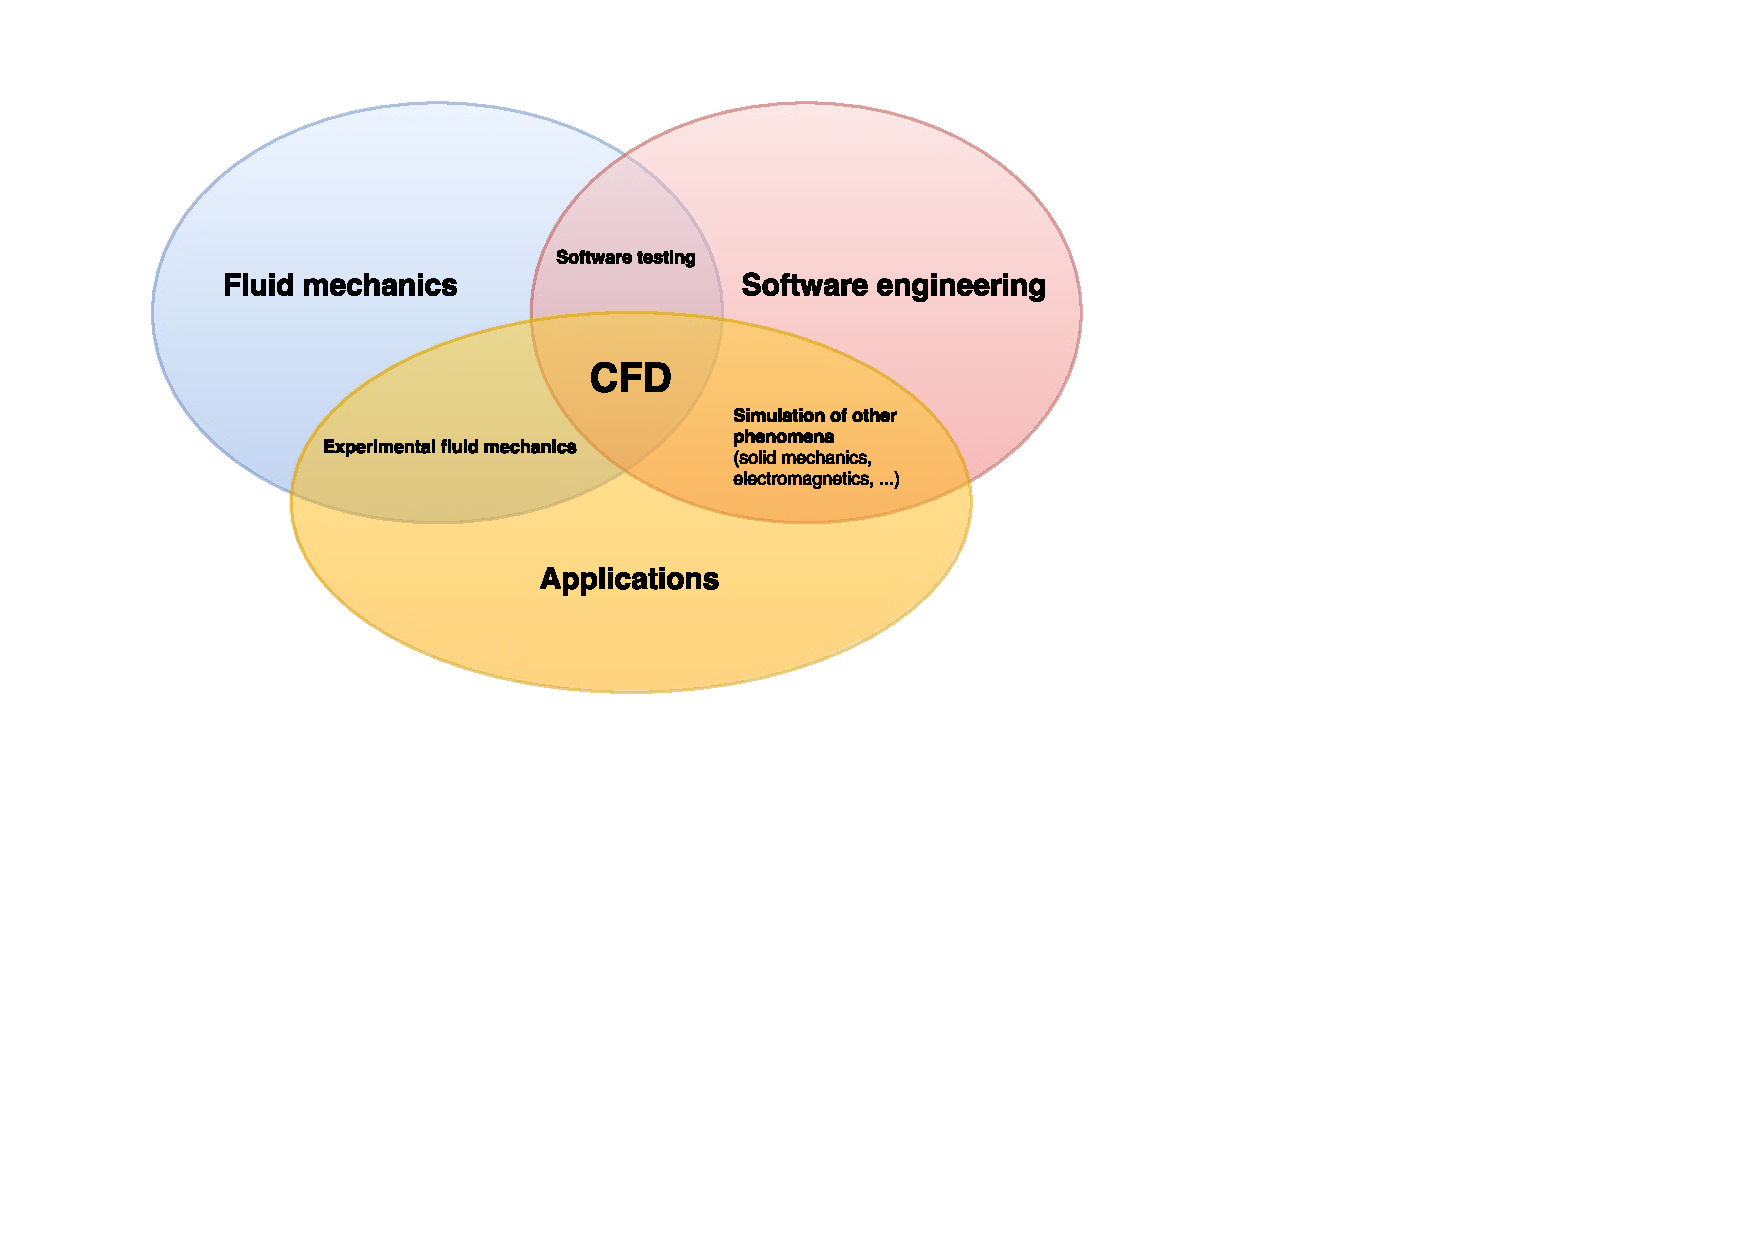
\includegraphics[trim=2cm 9cm 11cm 1cm,clip=true,width=0.7\textwidth]{Figures/Chapter1/CFD_scheme}
	\caption{Topics that conform CFD.}
	\label{fig-CFD}
\end{figure}

%Industrial problems
The CFD is widely used in many disciplines and industries like in the aerospace, automotive, chemical manufacturing, power generation, petroleum exploration, medical research, meteorology or astrophysics. It is a very valuable tool since it let to reductions in the cost of production by reducing the need of physical experimentation, improving the products or optimizing the production processes. In Table \ref{table-CFD_applications} we enumerate some more specific applications of CFD simulations that are very usefull for different disciplines.
\begin{table}[h]
\centering
\begin{tabular}{ll}
\toprule
Field&Application\\
\midrule
\midrule
\multirow{8}{*}{Biomedical}&Heart pumping\\
&Blood flow\\
&Air flow in lungs\\
&Nose and sinus flows\\
&Cell-fluid interface\\
&Artificial organ design\\
&Cardiac valve design\\
&Life support systems\\
\midrule
\multirow{1}{*}{Electronics}&Cooling flow in electronic devices\\
\midrule
\multirow{6}{*}{Aerospace and automotive}&Aerodynamic shape optimization\\
&Aerodynamic loads computation\\
&Turbines\\
&Propulsion systems\\
&Airbag Deployment\\
&In-Cylinder Engine Flow\\
\midrule
\multirow{4}{*}{Energy and power industry}&Heat exchange modeling\\
&Wind turbines blade design\\
&Pulverized coal combustion\\
&Emission of NOx particles\\
\midrule
\multirow{4}{*}{Environmental}&Impact of industrial exhausts\\
&Fire and smoke in buildings and tunnels\\
&Natural ventilation systems design\\
&Meteorology prediction\\
\midrule
\multirow{4}{*}{Civil}&Effect of wind on structures\\
&Water flow in rivers\\
&Water management\\
\bottomrule
\end{tabular}
\caption{CFD applications.}
\label{table-CFD_applications}
\end{table}

There already are CFD codes, both commercial and open source, that have the potential to solve a very broad spectrum of flow problems. However, the developement of computational algorithms for the simulation of turbulent flows is still an open topic. Moreover, the improvement of accuracy, the reduction of computational time and the increase of accessibility are also ongoing objectives in CFD. It is true that the CFD has some limitations, but the economic value of industrial applications has been demonstrated in a variety of industries.

%FE methods as CFD
The simulation of fluid flows relies on the fact that we can define a mathematical model that describes the fluid motion. The governing equations of the fluid dynamics are the Navier-Stokes equations. Then, the CFD basically consists on approximate the solution of these equations. Many approximation techniques can be used to simulate fluid flows, the most common are the Finite Element (FE) method, the Finite Differences (FD) method or the Finite Volume (FV) method. All of them are methods that can approximate the solution of a fluid flow and vary in the way in which the spatial domain is dicretized. 

The FD method is based on the application of a local Taylor expansion to approximate the governing equations, but it can only be applied on a discretization constructed by a network of topological squares or hexahedras, depending on the spatial dimensions. On the other hand, FE and FV methods are not restricted by this condition and are more extended in the CFD world. The FV method is based on the approximation of the average integral value on a reference volume being one of the main strengths the ability to handle discontinuous solutions. Rather than an integral average, the FE method is based on pointwise approximations on a grid. In contraposition to FV, it allows the use of high-order approximations and has a strong mathematical foundation behind.

In this thesis the FE method will be considered to discretize in space the Navier-Stokes equations. In any case, it has to be highlighted that the FV method can be recovered with a particular definition of the FE method.

%Exascale computing
The increasing computing power is one of the points that make not only the CFD, but also the computational mechanics in general, more appealing to solve engineering problems with more and more complexity. In order to take advantage of the continuously growing computational power acquired with the new improvements on super-computers, an advance in software design is imperative. New algorithms need to be designed to be used in the exascale computing environment. 

We understand by exascale computing the capacity of a computing system to perform at least one exaFLOPS ($ 10^{18} $ floating point operations per second). This computing capacity is still far from the current computer power, but many effords are dedicated to achieve this objective, which is expected to be acomplished before 2020. There are many issues in the High Performance Computing (HPC) community to be addressed in order to achieve the exascale goal. Some of them are related to the hardware development, including improvements on processors, memory size, memory bandwidth and energy consumtion. Furthermore, there is the need of software improvement in such a way that exascale computing systems can be fully exploited.

Exascale computing is the key with wich we will be able to perform high-fidelity simulations of real world problems. Such simulations are a great challenge of computational physics and engineering, and can transform the computational science into a fully predictive science.

%Large scale solvers
We still do not know much details about how exascale computing systems will be, but there is a clear priority in what software development refers. This is the definition and implementation of algorithms able to scale in extremely large computing environments (machines of the order of some million-cores). We recall here that an scalable algorithm has the property to have a computational cost proportional to the size of the problem that is being solved. Other numerical issues that are thought to be needed to achieve exascale computations are the use of high-order methods which give more accurate results for a given problem size and the development of adaptive methods, which can improve the efficiency of the simulation.

The application of a FE method to a Partial Differential Equation (PDE) leads to a matricial system of equations that has to be solved using linear algebra tools. The development of large scale FE solvers is accomplished by the use of preconditioners that improve the resolution of such matricial system. The most known algorithmically scalable preconditioners are the MultiGrid (MG) preconditioner and the Domain Decomposition (DD) based preconditioners. Nevertheless, in order to reach extreme scalabilty, the algorithmical scalability of a preconditioner is not a sufficient condition, since an efficient implementation is needed. 

%COMFUS group
The development of algorithms and implementations of scalable preconditioners is a hot topic in the FE field, and one of the main topics of the COMFUS team. The COMFUS group is the group where this thesis has been developed, and its name is the acronym of 

% (COMFUS group) in different lines of research, all of them related with the Starting Grant project of the European Research Council (ERC) headed by professor Santiago Badia.The objective of the COMFUS group is to develop significant advances on the simulation of the technology needed for the nuclear fusion. 




%From a technological point of view, nuclear fusion is considered as a safe and clean source of energy. In order to satisfy the future and increasing energetic needs of the society, there is the necessity  of efficient energy sources with a low $CO_2$ discharge. The increasing demand of energy sources that satisfy these conditions make nuclear fusion a strategic commitment for the EU energetic future.
%
%To make this energy source feasible, there must be a huge industrial development of the technology needed for its generation. The significance of the development of such technology arises with the creation of plans and European commissions such as the European Commission in the European Fusion Programme. This programme controls the construction and its subsequent experimentation of the experimental reactor ITER (International Thermonuclear Experimental Reactor). ITER will not be a completed fusion reactor, but it will allow to validate different concepts and technology needed to achieve the first fusion reactor able to provide energy efficiently, DEMO (DEMOnstration power plant). It is expected that ITER will be partially operative in 2017, but some tests such as the Tritium extraction will not be able to be performed until 2027. This date is too far given that the DEMO reactor is expected to be operative in the 2040 decade. This disadvantage explains the increasing need of numerical tools able to simulate the physical processes that occur in the nuclear fusion reactor. For instance, the European commission for the nuclear fusion development, Fusion for Energy (F4E), is opening constantly new calls for numerical investigations that allow the development of the needed technology. Currently, F4E is collaborating with the group where this thesis is being developed (COMFUS group) in different lines of research, all of them related with the Starting Grant project of the European Research Council (ERC) headed by professor Santiago Badia. 
%
%The objective of the COMFUS group is to develop significant advances on the simulation of the technology needed for the nuclear fusion. In this direction, the thesis is planed over the line of the development of numerical algorithms and computational tools able to simulate unsolved technological problems such as: 1) the plasma disruptions and magnetic confinement for large tokamaks and 2) the neutron shielding and the Tritium extraction inside the Test Blanket Modules (TBM). 

\section{Thesis objectives}

Residual-based VMS as LES

Mixed VMS formulations for LES

High-order FE methods

High-order time integration methods

Segregation of velocity-pressure

Adaptive time integration schemes

Large scale FE solvers

Scalable solvers

Application

The TBMs that wrap the fusion reactor core are a fundamental part of it. These modules not only are the responsible of the shielding that absorb the neutrons that emerge from the plasma, but also are the place where the Tritium is extracted. Tritium is needed to keep the plasma and it can not be found in nature, so its extraction is a key step. One of its design consists on a micro-channel system full of  liquid metal. Because of the magnetic forces that confine the plasma inside the reactor core, this liquid is subjected to the magnetohydrodynamics (MHD) equations.

As said before, these components can not be tested in ITER before 2027. When this occurs, its configuration will not be the same that the needed for the DEMO reactor. Then, the tests done in ITER reactor will mainly be used as a validation of the numerical simulation codes that will be used in the final design of the TBMs for the DEMO reactor.

These conditioning aspects imply that the research on numerical simulations able to reproduce such processes are a key step in the development of the nuclear fusion energy. In this thesis project we will continue the work of the COMFUS group in this line.

The liquid metals are electrical conductors that are subjected to the MHD physical laws, which couple the Navier-Stokes equations with Maxwell equations. These flows have a particular behaviour due to the magnetic effects. For a low magnetic Reynolds, the energy spectra is different of the defined by the classical flow theory. For this reason, it is necessary to \emph{develop numerical models able to simulate the quasi2D turbulence} that appears in these processes.

The stabilized finite element formulation for incompressible MHD, tested in laminar regime, that will be used in this thesis has been proposed recently by the group where this thesis is developed. The main novelty with respect to existent formulations is the use of the same interpolation for the fluid-dynamic and magnetic problems, keeping the optimal convergence. At this point, we want to explore its extension to turbulent cases by the use of Variational MultiScale (VMS) methods. These methods arise as a numerical stabilization techniques, but also model successfully the classical flow turbulence since they introduce numerical dissipation efficiently. Therefore, we firstly will \emph{test these methods in classical turbulent flows} to verify their applicability to a more complex turbulent flows. From this point, we want to apply the same methods to simulate the liquid metal problem, which is influenced by the magnetic field, and reproduce accurately the quasi2D turbulence.

The applications we have in mind are extremely complex and require large computational resources. The largest supercomputers are distributed-memory machines with thousands of cores. It is a very hard task to efficiently run simulation codes on these platforms. It requires excellent implementations and robust solvers, based on efficient preconditioners and Krylov solvers. The COMFUS team is actively working in this area, and the FEMPAR code developed by the team has already proved excellent scalability results up to 30,000 cores. The solvers used by the team combine robust and scalable solvers for symmetric positive definite problems and block-preconditioning. This approach allows to deal with indefinite problems like the Stokes system and fluids at low Reynolds numbers. However, there is still the challenge to scale up nonsymmetric and indefinite problems. In order to do so, we are forced to implement and \emph{develop novel techniques for nonsymmetric problems}.

The team has been actively working on new block preconditioners for inductionless and resistive MHD systems. These preconditioners, based on inexact-block LU factorizations, are used in combination with Krylov methods. Since these preconditioners are computationally intensive, it would be very appealing to use them as solvers instead of preconditioners. This approach, in the frame of resistive MHD has been exploited in \cite{badia_unconditionally_2012}, where the $\theta$ scheme was used for time integration. We plan to develop novel operator splitting methods based on implicit-explicit Runge-Kutta schemes. In particular, we want to \emph{design schemes that split velocity-pressure computations}.

Finally and related to the use of VMS methods, we want to \emph{test the advantages of the symmetric projection stabilization methods} with respect to classical VMS formulations.
%Besides to use these block preconditioners to solve the multiphysic problems, this thesis proposal also expect to use the block preconditioners structure to develop new time integrators which decouples the different physical problem variables. The idea is to take advantage of the Implicit-Explicit (IMEX) time integration technique using a Runge-Kutta scheme and operate with the different blocks to decouple the different physical fields that appears into the problem.
%
%\subsection{Large scale computation}
%As it has been said before, the physical processes that takes place in a nuclear fusion reactor lead to complex systems of equations. Besides the coupling between different physical problems, there also appear several length and time scales, resulting in a multi-scale problems. The way to solve accurately problems with large time scales without having numerical inestabilities and without using a small really time step, is by implicit methods. However, these methods require to solve nonlinear systems at each time-step. Then, there arise the need to use scalable solvers for massivelly parallel computers.
%
%It has to be said that the COMFUS group has an extensive experience in this topic. The code that will be used by the thesis development is designed to be used in distributed computers and it incorporates domain decomposition (DD) methods optimal for large scale problems that can be combined in a natural way with block preconditioners. The scalability of these methods has been proved to be excellent until 4096 CPUs {\color{red}(o mes??)}.
%
%To this end, this thesis project considers:
%\begin{itemize}
%\item {\bf Block preconditioners implementation and computational aspects}. As was said before, the multiphysical problem can be rewritten as a block system, i. e., one block for each unknown of the global problem. The non-diagonal blocks are those which couples the different subproblems. Here, the key decision is how to reorganize the system and subsequently how to define a good approximation to the original matrix, which will be used as a preconditioner. These preconditioners must be spectrally equivalent to the original matrix of the system of equations.
%
%{\color{red}... (Santi, queda alguna cosa a fer en aquest apartat? Em sembla que tot el que vam posar a la proposta de la FPU es lo que ja heu fet amb l'Alberto i el Ramon)}
%
%\item {\bf Domain Decomposition solvers for convection dominated flows}. {\color{red} ... (Aquest apartat no hi era a la proposta FPU, però l'he posat per mencionar lo del BDDC. Alguna idea per posar aqui?)}
%\end{itemize}

\section{Document structure}
 
% PRELIMINARIES

\chapter{Preliminaries}
\label{chap-Preliminaries}

%----------------------------------------------------------------------------------------

% Define some commands to keep the formatting separated from the content 
\newcommand{\keyword}[1]{\textbf{#1}}
\newcommand{\tabhead}[1]{\textbf{#1}}
\newcommand{\code}[1]{\texttt{#1}}
\newcommand{\file}[1]{\texttt{\bfseries#1}}
\newcommand{\option}[1]{\texttt{\itshape#1}}

%----------------------------------------------------------------------------------------

\section{The Governing equations of Fluid Mechanics}
\label{sec-C2_gov_eq}
In this section we will briefly state the basic concepts that one has to know about fluid mechanics and its mathematical description, which will be used in the forthcoming chapters.

Let us start with a review of the equations that govern the fluid flow. In this thesis we will restrict to constant-property Newtonian fluids. 

\subsection{The momentum equation}
\label{subsec-momentum}
From the Newton's second law, the momentum equation relates the fluid particle acceleration, $\frac{D\u}{Dt}$, to the external forces acting on such fluid particle. The external forces can be decomposed into the surface forces and the body forces, $\f$. The surface forces are described by the stress tensor $\boldsigma(\x,t)$ that is symmetric and, for constant-property Newtonian fluids, is defined by
\begin{equation}
\label{eq-stress_tensor_def}
\boldsigma = -\breve{p}\boldI + 2\mu\boldsymbol{\varepsilon}(\u), 
\end{equation}
where $\breve{p}$ is the pressure field, $\boldI$ the identity tensor, $\mu$ the viscosity, $ \u $ the fluid velocity and $\boldsymbol{\varepsilon}(\u)$ the strain rate tensor, which is defined by the following expression
\begin{equation}
\label{eq-strain_tensor_def}
\boldsymbol{\varepsilon}(\u)=\frac{1}{2}\left[\nabla\u+\left(\nabla\u\right)^T\right].
\end{equation}

The acceleration of the fluid particle is caused by the external forces according to the momentum equation
\begin{equation}
\label{eq-momentum_equation_def1}
\rho\frac{D\u}{Dt}=\nabla\cdot\boldsigma+\rho\f,
\end{equation}
being $\rho$ the density of the flow. Introducing the definition of the stress tensor \Eq{stress_tensor_def} into \Eq{momentum_equation_def1}, and dividing by the density $\rho$, which we consider to be constant, we get an alternative expression of the momentum equation
\begin{equation}
\label{eq-momentum_equation_def2}
\frac{D\u}{Dt}=-\nabla p+\nabla\cdot(2\nu\boldsymbol{\varepsilon}(\u))+\f,
\end{equation}
where we have used that $(1/\rho)\nabla\breve{p}=\nabla(\breve{p}/\rho)=\nabla p$, being $p:=\breve{p}/\rho$ the kinematic pressure, and $\nu=\mu/\rho$ the kinematic viscosity.

\subsection{Mass conservation}
\label{subsec-mass_conservation}
Matching the rate of change of mass in a given volume and the net mass flux across the boundary of such volume, and using the divergence theorem, we get the mass conservation or continuity equation, which is given by 
\begin{equation}
\label{eq-continuity_equation_def1}
\frac{\partial\rho}{\partial t}+\nabla\cdot(\rho\u)=0,
\end{equation}
which for constant density can be simplified to the kinematic condition that the velocity field be solenoidal or, what is the same, divergence-free:
\begin{equation}
\label{eq-continuity_equation_def2}
\nabla\cdot\u=0.
\end{equation}
Equation \Eq{continuity_equation_def2} is also called incompressibility constraint, since it is a constraint on the fluid velocity.

\subsection{Navier-Stokes equations}
\label{subsec-NS_equations}
Let $\Omega$ be a bounded domain of $\mathbb{R}^d$, where $d=2,3$ is the number of space dimensions, $\Gamma=\partial\Omega$ its boundary and $(0,T]$ the time interval. The strong form of the steady Navier-Stokes problem that govern the fluid flow motion consists of finding the velocity field $\u$ and the pressure field $p$ such that 
\begin{align}
\label{eq-NS_strong_momentum}
\frac{\partial\u}{\partial t}+\u\cdot\nabla\u-\nu\Delta\u+\nabla p=\f&\quad\mbox{in }\Omega\times(0,T],\\
\label{eq-NS_strong_continuity}
\nabla\cdot\u=0&\quad\mbox{in }\Omega\times(0,T],
\end{align}
where the decomposition of the velocity material derivative into the temporal partial derivative plus the convective derivative, $\frac{D\u}{Dt}=\frac{\partial\u}{\partial t}+\u\cdot\nabla\u$, and the fact that the velocity field is solenoidal have been used to simplify the momentum equation \Eq{momentum_equation_def2} into \Eq{NS_strong_momentum}. In forthcoming sections, the temporal partial derivative $ \frac{\partial(\cdot)}{\partial t} $ will also be denoted as $ \partial_t(\cdot) $.

Equations \Eq{NS_strong_momentum} and \Eq{NS_strong_continuity} need to be supplied with appropriate boundary and initial conditions. The boundary $\Gamma$ is divided into the Dirichlet ($\Gamma_D$) and the Neumann ($\Gamma_N$) parts such that $\Gamma_D\cup\Gamma_N=\Gamma$ and $\Gamma_D\cap\Gamma_N=\emptyset$. Then, the boundary and initial conditions can be written as
\begin{align}
\label{eq-NS_strong_Dir}
\u&=\u_g&\mbox{on $\Gamma_D\times(0,T]$,}\\
\label{eq-NS_strong_Neu}
(-p\mathbf{I}+\nu(\nabla\u+\nabla\u^T))\cdot\mathbf{n}&=\mathbf{t}_N&\mbox{on $\Gamma_N\times(0,T]$,}\\
\label{eq-NS_strong_Ini}
\u(\x,0)&=\u_0(\x)&\mbox{in $\Omega\times\{0\}$,}
\end{align}
$\mathbf{n}$ being the unit outward vector normal to $\Gamma$. For a solid wall, the velocity field on the Dirichlet boundary $\Gamma_D$ is governed by two conditions. The first of them is the no penetration condition, the flow cannot penetrate the wall.
\begin{equation}
\label{eq-NS_no_penetration}
\u\cdot\n=0\quad\mbox{on $\Gamma_D\times(0,T]$}.
\end{equation} 
For the tangential velocity components we impose the so called no-slip condition, which means that there is no relative movement between the wall and the fluid.
\begin{equation}
\label{eq-NS_no_slip}
\u\cdot\t=0\quad\mbox{on $\Gamma_D\times(0,T]$},
\end{equation}
being $\t$ a unit vector tangential to the wall. Putting together equations \Eq{NS_no_penetration} and \Eq{NS_no_slip} we have that $\u=\mathbf{0}$ on $\Gamma_D\times(0,T]$. If the wall is moving with a velocity $\u_g$ we recover the Dirichlet boundary condition \Eq{NS_strong_Dir}.

\subsection{Pressure and mass conservation}
\label{subsec-pressure_mass_conservation}
Let us now focus on the role that pressure field has in the fluid flow equations. If we take the divergence of the momentum equation \Eq{NS_strong_momentum}, assuming that the continuity equation \Eq{NS_strong_continuity} is not satisfied ($\nabla\cdot\u=\epsilon$), we have
\begin{equation}
\label{eq-NS_div_momentum}
\left(\frac{\partial}{\partial t}-\nu\Delta\right)\epsilon=-\Delta p-\nabla\cdot(\u\cdot\nabla\u).
\end{equation}
Considering problem \Eq{NS_div_momentum} with the initial condition $\epsilon_0=0$, we can say that the velocity field will be solenoidal ($\epsilon=0$) if, and only if, the following Poisson problem is satisfied
\begin{equation}
\label{eq-NS_poisson}
\Delta p=-\nabla\cdot(\u\cdot\nabla\u).
\end{equation}
Hence, we can state that the satisfaction of the Poisson problem \Eq{NS_poisson} is a necessary and sufficient condition for a solenoidal velocity field to remain solenoidal, see~\cite{pope_turbulent_2000}. Furthermore, for infinite domains, the solution of \Eq{NS_poisson} using the Biot-Savart law is given by 
\begin{equation}
\label{eq-NS_poisson_solution}
p(\x,t)=\frac{1}{4\pi}\int_\Omega\frac{\nabla\cdot(\u(\mathbf{y},t)\cdot\nabla\u(\mathbf{y},t))}{|\x-\mathbf{y}|}d\mathbf{y}.
\end{equation}
An important consequence of \Eq{NS_poisson_solution} is that the pressure field is non-local, that means that a fluctuation at one point $\mathbf{y}$ affects to the hole domain. A direct repercussion of the non-locality of the pressure is that the pressure waves sent from $\mathbf{y}$ induce far-field pressure forces ($-\nabla p$) that can agitate the fluid motion at large distances from that point. Then, every part of the flow feels every other part. This consequence is more relevant in the case of turbulent fluid flows, where eddies at different locations of the flow can interact each other. 


\section{The function spaces}
\label{sec-C2_functional_spaces}
Before describing the variational formulation of Navier-Stokes equations we need an introduction to some functional spaces. In this section we define the notation used in following sections and we give some definitions of fundamental function spaces. A deeper explanation of the concepts introduced in this section can be found in any functional analysis text, for example we refer to \cite{temam}, where we find a numerical analysis for the Stokes and Navier-Stokes equations.

Let us start considering $\Omega$ to be an open set of $\mathbb{R}^n$ with boundary $\Gamma$. Otherwise stated, we assume that the boundary of $\Omega$ is locally Lipschitz. We denote by $L^p(\Omega)$, with $1<p<+\infty$ (or $L^\infty(\Omega)$), the space of real functions defined on $\Omega$ with the $p$-th power absolutely integrable (or essentially bounded real functions for the case $p=\infty$). This is a Banach space with the norm 
$$\|\u\|_{L^p(\Omega)}:=\left(\int_\Omega|\u(\x)|^pd\Omega\right)^{\frac{1}{p}}$$
(or, for $p=\infty$,
$$\|\u\|_{L^\infty(\Omega)}:=\underset{\Omega}{\mbox{ess. sup}}|\u(\x)|).$$
For $p=2$, $L^2(\Omega)$ is a Hilbert space with the scalar product
$$(\u,\v)_\Omega:=\int_\Omega\u(\x)\v(\x)d\Omega.$$
Henceforth, when considering the scalar product over all domain $\Omega$ we will exclude the subscript, reading $(\cdot,\cdot)$. Furthermore, in forthcoming sections, the $L^2(\Omega)$-norm will be simply denoted as $\|\cdot\|$.
The Sobolev space  $W^{m,p}(\Omega)$ is the space of functions in $L^p(\Omega)$ with derivatives of order less than or equal to $m$ in $L^p(\Omega)$, being $m$ an integer and with $1\leq p\leq+\infty$. This is a Banach space with the norm
$$\|\u(x)\|_{W^{m,p}(\Omega)}:\left(\sum_{j\leq m}\|D^j\u(\x)\|^p_{L^p(\Omega)}\right)^{\frac{1}{p}},$$
where $D^j$ is the differentiation operator. When $p=2$, $W^{m,2}(\Omega)=H^m(\Omega)$ is a Hilbert space with the scalar product
$$(\u,\v)_{H^m(\Omega)}:=\sum_{j\leq m}\left(D^j\u,D^j\v\right).$$
Often we are concerned about $n$-dimensional vector functions with components in one of the spaces defined above. In this case we use bold characters to denote a vectorial space
$$\Lbf^p(\Omega):=\{L^p(\Omega)\}^n,\quad\Hbf^m(\Omega):=\{H^m(\Omega)\}^n.$$

Let $\Dcal(\Omega)$ be the space of $\Ccal^\infty$ functions with compact support contained in $\Omega$. The closure of $\Dcal(\Omega)$ in $H^m(\Omega)$ is denoted by $H^m_0(\Omega)$. The space $H^m_0(\Omega)$ can be though as the space of functions that belong in $H^m(\Omega)$ that vanish on the boundary $\Gamma$ in a general sense. Functions that belong to $H^m_0(\Omega)$ satisfy the Poincaré inequality
\begin{equation}
\label{eq-Poincare_inequality}
\|u\|\leq c(\Omega)\|\nabla\u\|,\quad\forall\u\in\Hbf^m_0(\Omega).
\end{equation}

From a physical point of view, as noticed in \cite{Foias}, we can think on the space $\Lbf^2(\Omega)$ as the space of all vector fields $\u$ with finite kinetic energy. Moreover, the $\Hbf^1(\Omega)$ can be though as the space of all vector fields $\u$ with finite enstrophy.

Let us consider some additional spaces that are useful in the mathematical description of the Navier-Stokes equations. A possible way to deal with the incompressibility constrain \Eq{NS_continuity} is to consider a functional space with less regularity than $\Hbf^1(\Omega)$ defined as
$$\Hbf(div,\Omega):=\{\u\in\Lbf^2(\Omega)|\nabla\cdot\u\in\Lbf^2(\Omega)\},$$
which is a Hilbert space with the norm
$$\|\u\|_{div}:=\|\u\|+\|\nabla\cdot\u\|.$$
The closure of $\Dcal(\Omega)$ in $\Hbf(div,\Omega)$ is denoted by $\Hbf_0(div,\Omega)$.
...

\subsection{The set $\Omega$}

\subsection{$L^p$ and Sobolev spaces}

\subsection{}

\section{The variational formulation}
\label{sec-C2_variational}
\subsection{Continuous formulation}
\label{subsec-variational_continuous}
Let us consider the strong form of the Navier-Stokes problem \Eq{NS_strong_momentum}-\Eq{NS_strong_Ini}. In order to formulate the equivalent variational problem we define a set of variational spaces that incorporates the homogeneous Dirichlet boundary condition and the temporal evolution
\begin{align}
\label{eq-C2_varia_NS_u_space}
&\mathcal{V}_g:=\left\{\v\in\Hbf^1(\Omega):\left.\v\right|_{\Gamma_D}=\u_g\right\}\equiv\Hbf^1_g(\Omega),\\
\label{eq-C2_varia_NS_v_space}
&\mathcal{V}_0:=\left\{\v\in\Hbf^1(\Omega):\left.\v\right|_\Gamma=0\right\}\equiv\Hbf^1_0(\Omega),\\
\label{eq-C2_varia_NS_p_space}
&\mathcal{Q}:=\Lbf^2(\Omega)/\mathbb{R}.
\end{align}
Given sufficiently smooth functions $ \v\in\mathcal{V}_0 $ and $ q\in\mathcal{Q} $, we obtain the variational or weak version of the Navier-Stokes equations multiplying \Eq{NS_strong_momentum} by $ \v $  and \Eq{NS_strong_continuity} by $ q $, integrating over $ \Omega $ and integrating by parts the second order derivatives. Then the variational Navier-Stokes problem reads: find $ \u\in\Lbf^2(0,T;\mathcal{V}_g),\\ $ and $ p\in\Lbf^1(0,T;\mathcal{Q}) $ such that: 
\begin{align}
\label{eq-C2_varia_NS_weak_momentum}
(\partial_t\u,\v)+\left(\nu\left(\nabla\u+\nabla\u^T\right),\nabla\v\right)+b(\u,\u,\v)+(\nabla p,\v)=&\left\langle f,\v\right\rangle&\forall\v\in\mathcal{V}_0,\\
\label{eq-C2_varia_NS_weak_continuity}
(\nabla\cdot\u,q)=&\ 0&\forall q\in\mathcal{Q}.
\end{align}
Adding up equations \Eq{C2_varia_NS_weak_momentum}-\Eq{C2_varia_NS_weak_continuity} we obtain an alternative weak form of the incompressible Navier-Stokes problem \Eq{NS_strong_momentum}-\Eq{NS_strong_Ini} consists, e.g., in finding $[\u,p]\in {L}^2(0,T;\mathcal{V}_g)\times {\cal D}'(0,T;\mathcal{Q})$ (distributions in time with values in $\mathcal{Q}_0$) such that
\begin{equation}
\label{eq-C2_NS_weak}
(\partial_t\u,\v) + B(\u;[\u,p],[\v,q]) = \left<\f,\v\right> 
\quad\quad\forall\v\in\mathcal{V}_0,\quad\forall q\in\mathcal{Q},
\end{equation}
satisfying the initial condition \Eq{NS_strong_Ini} in a weak sense. Here the form $B({\a};[\u,p],(\v,q))$ is defined as 
\begin{equation}
\label{eq-C2_bilinear}
B(\a;[\u,p],[\v,q]):=\nu(\nabla\u,\nabla\v)+b(\a,\u,\v)-(p,\nabla\cdot\v)+(q,\nabla\cdot\u)
\end{equation}
where the trilinear weak form of the convective term $b(\u,\v,\w)$ can be written in the following three equivalent ways
\begin{align}
\label{eq-C2_b_noskew}
&b(\u,\v,\w)=(\u\cdot\nabla\v,\w)&&\mbox{Non conservative},\\
\label{eq-C2_b_skew1}
&b(\u,\v,\mathbf{w})=\frac{1}{2}(\u\cdot\nabla\v,\mathbf{w})-\frac{1}{2}(\v,\u\cdot\nabla\mathbf{w})&&\mbox{Skew-symmetric (type 1)},\\
\label{eq-C2_b_skew2}
&b(\u,\v,\mathbf{w})=(\u\cdot\nabla\v,\mathbf{w})+\frac{1}{2}(\v\cdot\mathbf{w},\nabla\cdot\u)&&\mbox{Skew-symmetric (type 2)}.
\end{align}
Note that in the trilinear weak forms \Eq{C2_b_noskew}-\Eq{C2_b_skew2} the boundary integral terms that arise from the integration by parts have been neglected. This assumption is valid when strong Dirichlet boundary conditions are considered over all the boundary. Despite of that, this equivalence is lost at the discrete level. The skew-symmetric form (type 2) (\ref{eq-C4_b_skew2}) is very common when numerical analysis are presented ~\cite{badia_convergence_2014,burman_galerkin_2009,guermond_faedogalerkin_2007} but the skew-symmetric form (type 2) (\ref{eq-C4_b_skew1}) has important advantages when the first argument is a discontinuous function, as will be shown in forthcoming chapters.

The well-posedness of problem \Eq{C2_NS_weak} relies on the called LBB condition, which stands for the name of the authors that developed works related to that condition. See the works by Ladyzhenskaya ~\cite{ladyzhenskaya1969mathematical}, Babu\^{s}ka ~\cite{babuska_error-bounds_1971} and Brezzi ~\cite{brezzi1974existence}. The LBB condition is also called \textit{inf-sup} condition and reads as follows: there exist a positive constant $ \beta $ such that,
\begin{equation}
\label{eq-C2_lbb}
\inf_{q\in\mathcal{Q}}\sup_{\v\in\mathcal{V}_0}\frac{(\nabla\cdot\v,q)}{\|\v\|_\mathcal{V}\|q\|_{\mathcal{Q}/\ker A^t}}\ge\beta>0,
\end{equation}
being $ A^t $ the adjoin of the operator defined as 
\begin{equation}
\label{eq-C2_lbb_operator}
A: \mathcal{V}_0\rightarrow\mathcal{Q'} \quad| \quad\langle A(\v),a\rangle_{\mathcal{Q'}\times\mathcal{Q}}=(\nabla\cdot\v,q)\quad\quad\forall\v\in\mathcal{V}_0,\quad\forall q\in\mathcal{Q}
\end{equation}

\subsection{The Finite Element method}
\label{subsec-variational_finite_element}
In order to approximate the solution of the variational problem \Eq{C2_NS_weak}, one needs to construct finite-dimensional spaces in which the solution can be computed. The approach followed in this work to construct such finite-dimensional spaces is the called Finite Element (FE) method. According to Ciarlet, see ~\cite{ciarlet_finite_1978}, we can define a FE as follows.

Let $ K\subseteq\Rbb^n $ be a bounded closed set with nonempty interior and piece-wise smooth boundary, the element domain. Let $ \mathcal{S} $ be a finite-dimensional space of functions on $ K $, the space of shape functions. Let $ \mathcal{N}=\{\mathcal{N}_1,\mathcal{N}_2,...,\mathcal{N}_k\} $ be a basis for $ \mathcal{S}' $, the set of nodal variables. Then, $ (K,\mathcal{S},\mathcal{N}) $ is called a FE.

We refer to Brenner et al ~\cite{brenner_mathematical_2007} for a deeper explanation of the FE definitions.

In this thesis we will mainly use FE spaces composed by quadrilateral finite elements built from a tensor product of polynomials. For the 3D case, we consider a reference FE $ (\widetilde{K},\widetilde{\mathcal{S}},\widetilde{\mathcal{N}}) $ with $ \widetilde{K} $ a cube defined in $ [-1,1]^3 $, $ \widetilde{\mathcal{S}}=Q_k $ being
$$ Q_k:=\left\{\sum_jc_jp_j(x)q_j(y)r_j(z):\mbox{ with $ p_j $, $ q_j $ and $ r_j $ polynomials of degree $j \leq k $}\right\}, $$
and $ \widetilde{\mathcal{N}} $ denoting the point evaluations at $ \left\{(t_l,t_m,t_n):\ l,m,n=0,1,...,k \right\} $ where \\$\left\{-1 = t_0 < t_1 < ... < t_k = 1 \right\}$.

Let us now consider a FE partition $ \mathcal{T}_h $ of the domain $ \Omega $ composed by a set of elements $ \left\{K_e\right\}_{e=1}^{ne} $, being $ ne $ the total amount of elements in the domain. Let us consider $ F_K $ a mapping from $ K $ to $ \widetilde{K} $, i. e. $ F_K(K)=\widetilde{K} $ with its pull-back map defined as $ F^*_K(\hat{f}):=\hat{f}\circ F_K $, see ~\cite{ciarlet_general_1972,brenner_mathematical_2007} for more details on equivalence between FE.

Then the FE spaces for the velocity and pressure fields equivalent to \Eq{C2_varia_NS_u_space}-\Eq{C2_varia_NS_p_space} can be defined as
\begin{align}
\label{eq-C2_varia_NS_vh_space}
&\mathcal{V}_{h}:=\left\{\v_h\in(\mathcal{C}^0(\Omega))^d:\left.\v_h\right|_K=\tilde{\v}\circ F_K^{-1},\ \tilde{\v}\in(Q_{k_v})^d,\ K\in\mathcal{T}_h\right\},\\
\label{eq-C2_varia_NS_vgh_space}
&\mathcal{V}_{g,h}:=\left\{\v_h\in\mathcal{V}_h:\left.\v_h\right|_{K\cap\Gamma}=\u_g\right\},\\
\label{eq-C2_varia_NS_v0h_space}
&\mathcal{V}_{0,h}:=\left\{\v_h\in\mathcal{V}_h:\left.\v_h\right|_{\partial K}=0\right\},\\
\label{eq-C2_varia_NS_qh_space}
&\mathcal{Q}_h:=\left\{\mathcal{C}^0(\Omega)\cap\Lbf^2(\Omega)/\mathbb{R}:\left.q_h\right|_K=\tilde{q}\circ F_K^{-1},\ \tilde{q}\in Q_{kq},\ K\in\mathcal{T}_h \right\}.
\end{align}
Where $ k_v $ and $ k_q $, not necessarily equal, are the degree of the polynomials used to define the interpolation space for the velocity and pressure fields, respectively. In what follows, the subindex $ h $ will denote functions related to the FE space. Note that in this work both velocity and pressure field spaces, $ \mathcal{V}_h $ and $ \mathcal{Q}_h $, are considered to be made by continuous functions in the same partition of the domain, $ \mathcal{T}_h $.

\subsection{Semi-discrete formulation}
\label{subsec-variational_semidiscrete}
Let us consider a FE partition $ \mathcal{T}_h $ of the domain $ \Omega $ from which we can construct conforming finite dimensional spaces for the velocity $\mathcal{V}_{g,h}\subset\mathcal{V}_g$, and for the pressure $ \mathcal{Q}_{0,h}\subset\mathcal{Q}_0 $. The spaces $\mathcal{V}_{g,h}$ and $ \mathcal{Q}_{0,h} $ are the ones defined in the previous section, equations \Eq{C2_varia_NS_vgh_space} and \Eq{C2_varia_NS_qh_space} respectively.

The Galerkin FE approximation of \Eq{C2_NS_weak} consists in finding $[\u_h,p_h]\in {L}^2(0,T;\mathcal{V}_{g,h})\times {\cal D}'(0,T;\mathcal{Q}_h)$ such that
\begin{equation}
\label{eq-C2_NS_weak_discrete}
(\partial_t\u_h,\v_h) + B(\u_h;[\u_h,p_h],[\v_h,q_h]) = \left<\f,\v_h\right> 
\quad\quad\forall\v_h\in\mathcal{V}_{0,h},\quad\forall q_h\in\mathcal{Q}_h,
\end{equation}

Problem \Eq{C2_NS_weak_discrete} is well posed if the discrete \textit{inf-sup} condition equivalent to \Eq{C2_lbb} is satisfied. The discrete version reads: there exist a positive constant $ \beta_d $, independent of $ h $, such that,
\begin{equation}
\label{eq-C2_lbb_discrete}
\inf_{q_h\in\mathcal{Q}_h}\sup_{\v_h\in\mathcal{V}_{0,h}} \frac{(\nabla\cdot\v_h,q_h)}{\|\v_h\|_{\mathcal{V}_h}\|q\|_{\mathcal{Q}_h/\ker A_h^t}}\ge\beta_d>0,
\end{equation}
with $ A_h $ the equivalent operator to the one defined in \Eq{C2_lbb_operator}.



\section{The Variational Multiscale method}
\label{sec-C2_vms}
Let us consider a FE partition $\mathcal{T}_h$ of the domain $\Omega$ from which we can construct conforming finite dimensional spaces for the velocity $\mathcal{V}_{0,h} \subset \mathcal{V}_0$, and for the pressure $\mathcal{Q}_{0,h}\subset \mathcal{Q}_0$. 

It is well known that the Galerkin FE approximation \Eq{NS_galerkin} has numerical instabilities for high mesh Reynolds number problems, i.e., when the nonlinear convective term dominates the viscous term. Another drawback of that formulation is the discrete \textit{inf-sup} condition that must be satisfied by the pair $\mathcal{V}_{0,h} \times\mathcal{Q}_{0,h}$ in order to have a well-posed problem with bounded pressure. These difficulties are overcome by using the VMS approach, introduced by Hughes in \cite{hughes,hughes}, and that is stated as follows.

Let us consider a two-scale decomposition of spaces $\mathcal{V}_0$ and $\mathcal{Q}_0$ such that $$\mathcal{V}_0=\mathcal{V}_{0,h}\oplus\widetilde{\mathcal{V}}_0$$ and $$\mathcal{Q}_0=\mathcal{Q}_{0,h}\oplus\widetilde{\mathcal{Q}}_0,$$ where $\widetilde{\mathcal{V}}_0$ and $\widetilde{\mathcal{Q}}_0$ are infinite-dimensional spaces that complete the FE spaces in $\mathcal{V}_0$ and $\mathcal{Q}_0$, respectively. Hereinafter the subscript $(\cdot)_h$ will denote the FE component and the tilde $\widetilde{(\cdot)}$ the subgrid component. Applying the two-scale decomposition to \Eq{NS_weak} we obtain a discrete problem
\begin{align}
\label{eq-C2_vms_NS_discrete}
(\partial_t\u_h,\v_h)+(\partial_t\tilde{\u},\v_h)&+B(\a;[\u_h,p_h],[\v_h,q_h])\\\nonumber
&+\left(\tilde{\u},\mathcal{L}_{\a}^*(\v_h,q_h)\right)_h-\left(\tilde{p},\nabla\cdot\v_h\right)=\left<\f,\v_h\right>,
\end{align}
where $(\cdot,\cdot)_h=\sum_{K\in\mathcal{T}_h}(\cdot,\cdot)_K$ is the sum of scalar products (\ref{eq:scalar_product}) over each element $K$ of the partition $\mathcal{T}_h$, and
\begin{equation}
\label{eq-C2_vms_adjoint}
\mathcal{L}_{\a}^*(\v_h,q_h):=-\nu\nabla^2\v_h-\a\cdot\nabla\v_h-\nabla q_h
\end{equation}
is the formal of the adjoint operator of the momentum equation. The term involving the adjoint operator comes from an elementwise integration by parts of the terms involving the subscales, in which the boundary terms 
$\left( \v_{h},\nu \n\cdot \nabla \tilde{\u}\right)_{\partial h}$ and
$\left( q_{h},\n\cdot \tilde{\u}\right)_{\partial h}$
have been neglected (the subscript ${\partial h}$ is used to denote the sum over all elements of the integral on the boundary of each element). It also involves the approximation 
$b(\a,\tilde{\u},\u_h) \approx -(\tilde{\u},\a\cdot\nabla\v_h)$
which implies neglecting 
$\left( \v_{h},\n\cdot \a \tilde{\u}\right)_{\partial h}$ and
$(\tilde{\u},\nabla\cdot\a\v_h)$. 
These approximations are discussed in  \cite{codina_time_2007} together with the choice of $\a$ which defines the type of scale splitting (linear or nonlinear), also discussed below.

The discrete problem depends on $\tilde{\u} \in \widetilde{\mathcal{V}}_0$ and on $\tilde{p}\in \widetilde{\mathcal{Q}}_0$,  $\widetilde{\mathcal{V}}_0$ and $\widetilde{\mathcal{Q}}_0$ being infinite-dimensional. Therefore, the equations for $\tilde{\u}$ and $\tilde{p}$ obtained after applying the two-scale decomposition cannot be directly solved, but some modeling steps are needed to obtain a feasible method. Considering the subscale as a time-dependent variable of the problem (see below) and approximating the Navier-Stokes operator by two stabilization parameters $\tau_m^{-1}$ and $\tau_c^{-1}$ (see for example \cite{codina_time_2007}), the fine scale problem can be written as
\begin{align}
\label{eq-C2_vms_velo_sgs}
\partial_t\tilde{\u}+\tau_m^{-1}\tilde{\u}=\mathcal{P}(\R_u),\\
\label{eq-C2_vms_press_sgs}
\tau_c^{-1}\tilde{p}=\mathcal{P}(R_p).
\end{align}
In \Eq{velo_sgs}-\Eq{press_sgs} $\mathcal{P}$ denotes the projection onto the space of subscales, which is discussed below. In turn, the vector $\R$ is the residual of the Navier-Stokes equations \Eq{NS_strong_mome}-\Eq{NS_strong_inc}, defined as $\R=[\R_u,R_p]^T$, with
\begin{align}
\label{eq-C2_vms_Ru}
%&\R_u=\f-\left(\partial_t\u_h+N((\u_h+\tilde{\u}),\u_h)+\nabla p_h \right),\\
%&\R_u=\f-\left(\partial_t\u_h+ \a \cdot \nabla \u_h + \nabla p_h \right),\\
&\R_u=\f-\partial_t\u_h-\mathcal{L}_{\a}(\u_h,p_h),\\
\label{eq-C2_vms_Rp}
&R_p=-\nabla\cdot\u_h.
\end{align}
where
\begin{equation}
\label{eq-C2_vms_operator}
\mathcal{L}_{\a}(\v_h,q_h):=-\nu\nabla^2\v_h+\a\cdot\nabla\v_h+\nabla q_h
\end{equation}
%and $N((\u_h+\tilde{\u}),\u_h)=(\u_h+\tilde{\u})\cdot\nabla\u_h$ is the convective term. 
Finally, the expressions of the stabilization parameter $\tau_m$ is 
\begin{align}
\label{eq-C2_vms_tau_m}
&\tau_m=\left(\frac{c_1\nu}{h^2}+\frac{c_2|\a|}{h}\right)^{-1},
\end{align}
whereas we consider two possible definitions of $\tau_c$, viz. $\tau_c = 0$ (which implies $\tilde{p} = 0$) and 
\begin{align}
\label{eq-C2_vms_tau_c}
&\tau_c=\frac{h^2}{c_1\tau_m},
\end{align}
where $h$ is the mesh size and $c_1$ and $c_2$ are algorithmic constants. Let us comment on expression \Eq{tau_m}:
\begin{itemize}
\item The influence of the constants $c_1$ and $c_2$ is discussed in Section XXXX. A theoretical way to determine them would be to impose that the numerical dissipation they introduce be equal to the molecular dissipation in turbulent regimes, as explained in~\cite{guasch-codina-13}. 
\item The definition of $\tau_m$ in \Eq{tau_m} is not standard, in the sense that the one used often depends on the time step size of the time discretization, $\delta t$. Instead of \Eq{tau_m}, $\tau_m^{-1}=\frac{1}{\delta t} + \frac{c_1\nu}{h^2}+\frac{c_2|\a|}{h}$ is more often considered (see, e.g., \cite{Hsu2010,gamnitzer_time-dependent_2010}). We refer to 
Section XXXX~\ref{sec:small_time_step} for a more detailed discussion about this topic. Likewise, other expressions with the same asymptotic behavior in terms of $h$, $\nu$ and $|\a|$ can also be employed.
\item Expression \Eq{tau_m} corresponds to linear isotropic elements. If elements of order $p$ are used ($p$ is not the pressure, here), $c_1$ must be replaced by $c_1 p^4$ and $c_2$ by $c_2 p$. For anisotropic elements, the definition of $h$ within each element is not obvious. A possibility is explained in \cite{Principe2010}.
\end{itemize}

In the following three sections we discuss the particular ingredients of our VMS models. A different summary can also be found in \cite{Codina-chap-2011}, together with some numerical experiments. 

\subsection{The dynamics of the subscales}
\label{subsec-C2_vms_dyn}
Stabilized formulations were originally developed for steady convection-diffusion \cite{Brooks_1982} and Stokes \cite{Douglas_1989,Hughes_1986_5} problems. As the numerical instabilities have a spatial nature, the time dependency of the subscales was not considered, and the standard choice \cite{Hughes2000,hughes_large_2001,bazilevs_variational_2007} was to take 
\begin{equation}
\label{eq-C2_vms_static_sgs}
\tilde{\u}=\tau_m \mathcal{P}(\R_u),
\end{equation}
that is, to neglect the temporal derivative of the subscales in (\ref{eq:velo_sgs}). In this case, the subscales are called quasi-static in what follows.

The subscale as a time dependent variable of the problem was introduced in \cite{codina_stabilized_2002,codina_time_2007}. It gives rise to important properties like commutativity of space and time discretization, stability without restrictions on the time step size \cite{codina_time_2007,Badia2009a} and, combined with orthogonal subscales, to convergence towards weak solutions of the Navier-Stokes equations \cite{Badia2013Convergence} and the possibility of predicting backscatter \cite{Codina-chap-2011,Principe2009}. 

Equation \Eq{velo_sgs} can be analytically integrated to give
\begin{equation}
\label{eq:exact_sgs}
\tilde{\u}(t^*)=\tilde{\u}(0) + \mu^{-1}(t^*) \int_0^{t^*} \mu(t) \mathcal{P}\R_u {\rm d}t, \quad \quad \mu(s)=\exp \int_0^s \tau^{-1}(t){\rm d}t,
\end{equation}
where it is explicitly seen that the subscale is a function of the residual but also of the flow history. In practice this integration is performed numerically, as described below.

\subsection{(Non)linear scale splitting}
\label{subsec-C2_vms_nl}
The original VMS formulation \cite{hughes_multiscale_1995,hughes_variational_1998} was developed having linear problems in mind and its extension to the Navier-Stokes equations was implicitly based on a ``linearization'', fixing the advection velocity and applying the multiscale splitting to the rest of the terms. A nonlinear scale splitting was used in \cite{Hughes2000,hughes_large_2001} together with an explicit resolution of the small scales in which a Smagorinsky damping was introduced. A nonlinear scale splitting with modeled subscales was used in \cite{codina_stabilized_2002, bazilevs_variational_2007} and in \cite{codina_time_2007}, where it was shown that it leads to global conservation of momentum. We therefore consider both options
%The vector $\a$ appearing in (\ref{eq:bilinear}) and (\ref{eq:adjoint}) is the advection velocity of the convective term. It can be defined in two different ways depending if we use a linear or a nonlinear scheme for the subscales definition. That is, 
\begin{align}
\label{eq-C2_vms_a_lin}
&\a=\u_h&&\mbox{for linear subscales},\\
\label{eq-C2_vms_a_nl}
&\a=\u_h+\tilde{\u}&&\mbox{for nonlinear subscales}.
\end{align}

\begin{remark}
\label{rem-skewsym}
When we use the nonlinear definition for the advection velocity, $\a=\u_h+\tilde{\u}$, the skew-symmetric term \textit{type 2} \Eq{b_skew2} in the FE equation \Eq{NS_discrete} reads: 
\begin{equation}
\label{eq-C2_vms_b_skew2_aux1}
b(\a,\u_h,\v_h)=((\u_h+\tilde{\u})\cdot\nabla\u_h,\v_h)+\frac{1}{2}(\u_h\cdot\v_h,\nabla\cdot\u_h)+\frac{1}{2}(\u_h\cdot\v_h,\nabla\cdot\tilde{\u}).
\end{equation}
The last term is not well-defined, since it includes derivatives of the discontinuous subscale $\tilde{\u}$. One possibility is to neglect it (as previously done with other similar terms when arriving to \Eq{NS_discrete}), which implies
\begin{equation}
b(\a,\u_h,\u_h)=-\frac{1}{2}(|\u_h|^2,\nabla\cdot\tilde{\u}),
\end{equation}
the same result obtained when the non conservative form is used.
By contrast, the skew-symmetric term \textit{type 1} in the FE equation \Eq{NS_discrete} reads
\begin{equation}
\label{eq-C2_vms_b_skew1_aux1}
b(\a,\u_h,\v_h)=\frac{1}{2}((\u_h+\tilde{\u})\cdot\nabla\u_h,\v_h)-\frac{1}{2}((\u_h+\tilde{\u})\cdot\u_h,\nabla\cdot\v_h)
\end{equation}
from where
\begin{equation}
b(\a,\u_h,\u_h)=0.
\end{equation}
% and we can not use the FE shape function derivatives to approximate it because the subscales are on another space. Then we avoid this problem by neglecting this term. 
%Therefore, the skew-symmetric term \textit{type 2} implementation for a nonlinear definition of the subscales will be
%\begin{equation}
%\label{eq:b_skew2_aux2}
%b(\a,\u_h,\v_h)=(\a\cdot\nabla\u_h,\v)+\frac{1}{2}(\u_h\cdot\v_h,\nabla\cdot\a)-\frac{1}{2}(\u_h\cdot\v_h,\nabla\cdot\tilde{\u}).
%\end{equation}
In Subsection XXXX(\ref{subsec:result_DHIT}) we will see the influence of the two forms of the convective term on the results.
It is worth noting that the same approximations have been introduced in all cases to implement $b(\a,\tilde{\u},\u_h)$, but these approximations are taken into account in the (usual) energy estimates of Section XXXX\ref{sec:energy}.
%Note that \textit{type 2} is the standard choice.
\end{remark}

\begin{remark}
At the continuous level, the different expressions of the convective term are also equivalent to the so called conservation form
\begin{align}
b(\u,\v,\w)= -(\u\otimes \v,\nabla\w).\nonumber
\end{align}
In the discrete problem, the nonlinear scale splitting leads to the following terms in the momentum equation:
\begin{align}
b(\a,\u_h +\tilde\u,\v_h)= - (\u_h\otimes\u_h, \nabla\v_h)
- (\u_h\otimes\tilde\u, \nabla\v_h)- (\tilde\u\otimes\u_h, \nabla\v_h)
- (\tilde\u\otimes\tilde\u, \nabla\v_h).\label{eq:nonconconv}
\end{align}
Even if this is not exactly what we get using the non-conservative or skew-symmetric forms because of the approximation error, this allows us to interpret the different contributions arising from the nonlinear scale splitting. As it is explained in \cite{Codina-chap-2011}, from (\ref{eq:nonconconv}) we can identify the contributions from the cross stresses, the Reynolds stresses and the subgrid scale tensor. 
\end{remark}

\subsection{The space for the subscales}
\label{subsec-C2_vms_oss}
The selection of the space for the approximation of the subscales determines the projection $\mathcal{P}$ appearing in the right-hand side of \Eq{velo_sgs} and \Eq{press_sgs}. The first option, already considered in \cite{Hughes2000,hughes_large_2001,bazilevs_variational_2007} and named Algebraic Subgrid Scale (ASGS) in \cite{codina_stabilization_2000} is to take the subscales in the space of the residuals, that is,
%method is characterized by the following projection definition:
\begin{equation}
\label{eq-C2_vms_P_ASGS}
\mathcal{P}:=\mathbf{I}.
\end{equation}
Another possibility introduced in \cite{codina_stabilization_2000} is to consider the space of the subscales orthogonal to the FE space. The main motivation of the method is that a stability estimate for the projection onto the FE space of the pressure and/or the convective terms can already be obtained in the standard Galerkin method and therefore the only ``missing'' part is the orthogonal one. The Orthogonal Subscales (OSS) method is then characterized by the following projection definition:
\begin{equation}
\label{eq-C2_vms_P_OSS}
\mathcal{P}:=\Pi_h^\bot=\mathbf{I}-\Pi_h,
\end{equation}
where $\Pi_h$ is the projection onto the FE space. With this choice, the residual of the momentum equation does not depend on $\partial_t\u_h$. Likewise, $\mathcal{P}(\f)$ in this case is only well defined for $\f\in L^2(\Omega)^d$. In the case of minimum regularity, $\f\in H^{-1}(\Omega)^d$, this term can be simply neglected without upsetting the accuracy of the method.

In fact, with this choice, the orthogonality between the space of subscales and the FE space is only guaranteed when the stabilization parameters are constant. If this is not the case, the method is still optimally convergent \cite{Codina_2008a} but this property is lost. In order to have truly orthogonal subscales, \emph{which guarantees a proper separation of the FE and the subgrid scale kinetic energies} (see below and Section \ref{sec:energy}) a slight modification of the projection $\Pi_h$ is needed (see \cite{Codina_2008a}). We will use two different weighted projections: one for the velocity subscales ($\Pi_m$) in \Eq{velo_sgs} and another for the pressure subscales ($\Pi_c$) in \Eq{press_sgs}. We define the weighted projections $\Pi_m$ and $\Pi_c$ such that given any vector $\w\in\mathcal{V}_0$ and any scalar $r\in\mathcal{Q}_0$ we have
\begin{align}
\label{eq-C2_vms_Pi_tau_m}
&(\tau_m\Pi_m(\w),\v_h)=(\tau_m\w,\v_h)&&\forall\v_h\in\mathcal{V}_{0,h},\\
\label{eq-C2_vms_Pi_tau_c}
&(\tau_c\Pi_c(r),q_h)=(\tau_cr,q_h)&&\forall q_h\in\mathcal{Q}_{0,h}.
\end{align}
These definitions guarantee the orthogonality between the FE and subscale spaces in the case of static subscales, that is, neglecting temporal derivatives in \Eq{velo_sgs}. It then follows that the term containing the temporal derivative of the subscale in the FE equation \Eq{NS_discrete} also vanishes.

However, if the dynamic version of the method is used, the weight of the projection \Eq{Pi_tau_m} must be conveniently modified to ensure the mentioned orthogonality. As it can be seen in XXXXX(\ref{eq:exact_sgs}), the definition of the weight depends on the time integration strategy, as explicitly stated in Section XXXX\ref{sec:discrete}.

\section{Time integration}
\label{sec-C2_time_integration}
In this section, our aim is to state some basic concepts about the time discretization. Once we have defined the semi-discrete problem, as it has been formulated in Section \ref{subsec-variational_semidiscrete}, we end up with an Ordinary Differential Equation (ODE), which has to be integrated in order to get the solution of the problem.

In the current work we only will consider the called \textit{direct integration} methods. The \textit{direct integration} of the transient equations rely on a numerical step-by-step procedure, where the word \textit{direct} means that no transformation of the ODE problem is carried out a priori. Looking at the litarature, many techniques can be found based in this kind of procedure. For instance in \cite{bathe_finite_2006} the description of the following methods can be found: the central difference method, the Houbold method, the Newmark method or the $ \theta $-method. An exhaustive analysis of such methods can be found in \cite{belytschko_computational_1983}.

Other commonly used time integration methods in the computational fluid dynamics field are the Backward Differentiation Formulas (BDF), the generalized-$ \alpha $ method or the Runge-Kutta time integration schemes, see \cite{brayton_new_1972, jansen_generalized-alpha_2000, dettmer_analysis_2003,hairer_solving_2008} for instance.

Within the forthcoming chapters, only the $ \theta $-methods and Runge-kutta schemes are used to integrate in time the incompressible Navier-Stokes equations. Consequently, in the following subsections only these two methods are described. 

\subsection{$ \theta $-method}
Let suppose that we have an initial-value problem with first order ODE of the form
\begin{align}
\label{eq-C2_time_ODE}
&\frac{\partial u}{\partial t}=f(t,u),\quad\in(0,T)\\
\label{eq-C2_time_ODE_0}
&u(0)=u_0.
\end{align}
One of the most popular, widely used and simplest method to solve problem \Eq{C2_time_ODE}-\Eq{C2_time_ODE_0} are the so-called single step (one-step) schemes, particularly, the theta-method, which is usually denoted as $ \theta $-method. Using the notation $u(t_n) = u_n$, the $ \theta $-method is defined as
\begin{align*}
\label{eq-C2_time_theta_method}
&u_{n+1} = u_n + h (\theta f(t_{n+1}, u_{n+1}) + (1-\theta )f(t_n,u_n)),\\
&u(0) = u_0,
\end{align*}
being $ h $ the time step size and $ t_n = nh $ for $ n=0,...,N $, with $ N=T/h $. Here $ \theta \in [0, 1] $ is a fixed parameter. The $ \theta $-method is considered here as basic method since it represents the most simple Runge-Kutta method (and also linear multistep method). The case of $ \theta=0.5 $ is of second order and is called Crank-Nicolson method. For $ \theta=0 $ we have the so called (explicit) Forward Euler method and for $ \theta=1 $ the (implicit) Backward Euler (BE) method.

\subsection{Implicit-explicit Runge-Kutta schemes}
One of the main goals of this thesis is the construction of efficient solvers for the resolution of the incompressible turbulent Navier-Stokes equations. The solver efficiency can be addressed not only by the use of efficient time integrators, but also by the application of efficient algebraic solvers for the final discrete system of equations. In this direction, the time integration scheme can help to construct smaller systems of equation segregating the different variables that appear on the problem and allowing to solve efficiently each uncoupled variable separately.

In \Chap{SRK} and \Chap{SVMS} we will consider the application of Implicit-Explicit (IMEX) Runge-Kutta methods for the time integration of the Navier-Stokes equations. The aim is to take advantage of the IMEX schemes for Runge-Kutta methods to uncouple the pressure and velocity degrees of freedom when solving these equations. We also want to use the Runge-Kutta background to implement an adaptive time stepping technique to solve efficiently transient incompressible flow problems.

Given an ODE problem of the type
\begin{equation}
\label{eq-C2_time_ODE}
\frac{\partial u}{\partial t}=f(u)+g(u), 
\end{equation}
being $f$ and $g$ different operators which definition depends on the specific problem, an IMEX scheme consists of applying an explicit discretization for the operator $f$ and an implicit discretization for $g$. This approach comes from the fact that ODEs usually are composed by operators of different nature. For instance, thinking in the convection-diffusion problem we have two different operators, which represent the convection term (let us denote it by $f$) and the diffusion term (which we will denote as $g$). As it is well known, the convection term is often nonlinear (i.e. burgers equation) while the diffusion term is generally linear and stiff. When $f\equiv0$, problem (\ref{eq-C2_time_ODE}) results in a stiff and linear system, which is natural to be solved using an implicit scheme. Otherwise, if $g\equiv0$ the problem becomes nonlinear and it could be convenient to be solved using an explicit time integration scheme. Ascher et al. in \cite{ascher_implicit-explicit_1995} study some multistep IMEX methods for convection-diffusion problem type. Often these type of methods are used in conjunction with spectral methods, see \cite{canuto_spectral_1988, kim_application_1985}.

The IMEX approach can be used not only for multistep schemes, but also for Runge-Kutta time integration techniques. The multistage nature of the Runge-Kutta methods also make feasible IMEX schemes with even better properties than multistep methods, see \cite{ascher_implicit-explicit_1997} where some Runge-Kutta IMEX schemes are developed for the convection-diffusion problem.

The idea of the Runge-Kutta methods is to approximate the integral $u(t_{n+1})=u(t_n)+\int_{t_n}^{t_{n+1}}\left[f(u)+g(u)\right]\ dt$ using a numerical quadrature with the points $c_1,...,c_s$ and their weights $b_1,...b_s$, which leads to
\begin{equation}
\label{eq-C2_time_ODE_int}
u(t_{n+1})=u(t_n)+h\sum_{i=1}^sb_i\left(f(u(t_n+c_ih))+g(u(t_n+c_ih))\right)+\mbox{Error}.
\end{equation}

Hereafter we will write $t_i$ instead of $t_n+c_ih$. Suppose we have an approximation $u_n$ to $u(t_n)$); to use (\ref{eq-C2_time_ODE_int}) we also need values $u_i$ to put in for $u(t_i)$. We compute them also by numerical quadratures on the same nodes:
\begin{equation}
\label{eq-C2_time_RK_i}
u_i=u_n+h\sum_{j=1}^sa_{ij}\left(f(u_j)+g(u_j)\right).
\end{equation}
In general this is a set of implicit equations, which we solve and use in (\ref{eq-C2_time_ODE_int}) for our next value
\begin{equation}
\label{eq-C2_time_RK_n+1}
u_{n+1}=u_n+h\sum_{i=1}^sb_i\left(f(u_i)+g(u_i)\right).
\end{equation}

The formulation (\ref{eq-C2_time_RK_i})-(\ref{eq-C2_time_RK_n+1}) define a Runge-Kutta method, which we designate by displaying its coefficient in the called Butcher tableau:
\begin{equation}
\label{eq-C2_time_Butcher_tab}
\begin{array}{c|cccc}
c_1&a_{11}&a_{12}&...&a_{1s}\\
c_2&a_{21}&a_{22}&...&a_{2s}\\
\vdots&\vdots&\vdots&\ddots&\vdots\\
c_s&a_{s1}&a_{s2}&...&a_{ss}\\
\hline
 &b_1&b_2&...&b_s
\end{array}
\end{equation}

% Runge-Kutta for NSI
Runge-Kutta techniques have been widely used for a lot of ODE problem types. The Navier-Stokes semidiscrete problem is not an exception and the use of Runge-Kutta methods for its time integration can be easily found in the literature, e. g. \cite{nikitin_third-order-accurate_2006,sanderse_energy-conserving_2013,sanderse_accuracy_2012,sterner_semi-implicit_1997}. However, like the multistep methods, the Runge-Kutta schemes need to solve several systems of equations at each time step. Further, when we use an implicit scheme all stages could be coupled, resulting a large system of equations to be solved. This drawback can be bypassed using an explicit scheme which only needs to evaluate the operators that arise from the Navier-Stokes problem. But the use of an explicit scheme, as it is well known, involve a restriction in the time-step size in order to ensure stability, see for instance the chapter IV.2 in \cite{hairer_solving_1993}. 

Diagonally Implicit Runge-Kutta methods (DIRK) can be used to avoid stability problems and solving implicitly each Runge-Kutta stage uncoupledly, see \cite{alexander_diagonally_1977}. This technique consists on setting all the Butcher tableau values $a_{ij}$ in (\ref{eq-C2_time_Butcher_tab}) that are above the diagonal to zero. That is, $a_{ij} = 0$ for all $j>i$. In fact, in \cite{alexander_diagonally_1977} the use of the DIRK term is what in \cite{hairer_solving_1993} is referred by Singly Diagonally Implicit Runge-Kutta methods (SDIRK) which means that all the diagonal terms are equal, $a_{ii}=\gamma$. As pointed out by Alexander in \cite{alexander_diagonally_1977}, the use of SDIRK methods allow to use the same LU-factorization when solving repeatedly the multistage system of equations.

% Pressure segregation
An interesting issue when solving the transient Navier-Stokes problem is the decoupling of the velocity and pressure. There are several techniques to deal with this approach that consists on solving separately the velocity degrees of freedom and the pressure by approximating the coupling terms. One of them, for example, is the widely used Fractional step method, \cite{donea_finite_1982}. There also are some works done in this direction for multistep methods, see for instance \cite{kim_application_1985}. Nikitin in \cite{nikitin_third-order-accurate_2006} suggested a Runge-Kutta method which decouples pressure and velocity by using a pressure splitting technique on the last step of the scheme.

% Adaptivee time stepping
Also related with the time integration procedures, there appears the idea of using an adaptive time stepping technique. Adaptive time stepping is an interesting tool that allows to control the accuracy of the time integration, but also improves the simulation efficiency. In this direction, the Runge-Kutta method provides an excellent background to implement this computational tool since we can use the different stages to compute an error estimate at each time step. John et al. in \cite{john_adaptive_2010} studied some time stepping control methods applied to different types of integration schemes, including the DIRK scheme. A more specific step-control analysis for explicit and implicit Runge-Kutta methods is done in \cite{hairer_solving_1993}, where a predictive controller is also proposed. More adaptive time step techniques are proposed in \cite{gresho_adaptive_2008} for convection-diffusion equation and in \cite{kay_adaptive_2010} for the Navier-Stokes equations. Nikitin in \cite{nikitin_third-order-accurate_2006} also includes a section dedicated to the adaptive time step.


\subsection{Stability and order of convergence}
Some definitions of stability and order of convergence need to be introduced since it will be used to charachterize some of the methods used in forthcoming chapters. Deeper explanations on stability and order conditions can be found in \cite{hairer_solving_2008,hairer_solving_1993}.

When analysing stability of ODEs, the solution of the Dahlquist's equation $ u'=\lambda u $ is studied. After applying the implicit Euler method it reads
\begin{equation}
\label{eq-C2_Dahlquist}
u_1=u_0+h\lambda u_1,
\end{equation}
being $ h $ the step size. The solution to \Eq{C2_Dahlquist} is
\begin{equation}
\label{eq-C2_Dahlquist_sol}
u_1=R(h\lambda)u_0,
\end{equation}
where $ R(z) $ is called the stability function for $ z\in\mathbb{C} $. For $ \theta $-methods, the stability function reads $ R(z)=\frac{1+z(1-\theta)}{1-z\theta} $.

Under these definitions we say that a method is \textit{A-stable} if 
\begin{equation}
\label{eq-C2_A_stable}
z\in\mathbb{C}^-,\quad\mbox{with $\quad\mathbb{C^-}:=\{z\in\mathbb{C}|\ Re\ z\le0\} $}.
\end{equation}
It can be shown that a $ \theta $-method is A-stable for all $ \theta\ge\dfrac{1}{2} $, see \cite{lambert_numerical_1991}. Furthermore, we say that a method is \textit{L-stable} when it is A-stable and additionaly it satisfies
\begin{equation}
\label{eq-C2_L_stable}
\lim_{z\rightarrow\infty}R(z)=0.
\end{equation}

Let us consider a Runge-Kutta method given by equations \Eq{C2_time_RK_i}-\Eq{C2_time_RK_n+1}. We say that a Runge-Kutta method has \textit{order p} if 
\begin{equation}
\label{eq-C2_time_RK_order}
\|u(t_{n+1})-u_{n+1}\|\le Ch^{p+1}.
\end{equation}


\section{Conclusions}
\label{sec-C2_conclusions}

\chapter{The turbulence phenomena}
\label{chap-Turbulence}
One of the main topics of this thesis is the turbulence phenomena that appear in incompressible fluid flows. In order to put the reader in context, it worth describing the main properties and definitions of such kind of flows, albeit rather briefly. 

Some elementary definitions are established in the first section of this chapter. Thereafter, a short introduction to the vorticity is given, together with some characteristic properties of this field. The definition of the Reynolds stresses is stated subsequently, giving some insights of what does \textit{turbulence modelling} mean. In forthcoming chapters, some turbulent quantities will be used to characterize the fluid flow, so we dedicate some lines in this chapter on the explanation of such quantities. Finally, particular characteristics of isotropic turbulence and wall bounded turbulent flows are detailed. Here we introduce the turbulence tests performed during the thesis.

For a deeper explanation of turbulence phenomena we refer to \cite{pope,davidson,orlandi,tennekes,lesieur}.

\section{Introduction to turbulence}
\subsection{Elementary concepts}
In the comming chapters some elmentary conceps will be used. Here we give a brief definition of the most important ones:
\begin{itemize}
\item\keyword{Categories of fluid flow:}\\Fluid mechanics and fluid flows are often divided into different regimes. In particular, one can make three different sub-divisions. The first division distinguishes between fluids that may be treated as inviscid or fluids in where the finite viscosity must be taken into account. The second sub-division distingishes between laminar (organized) and turbulent (chaotic) flow. The final sub-division is between irrotational(or potential) flow and rotational flow.

In this thesis we will mainly focus on the second sub-division, distinguishing between laminar and turbulent flows. Except when stated, the fluid will be considered to be viscous and rotational.

\item\keyword{Newton's law of viscosity}\\In most fluids the shear stress is quantified using an empirical law known as Newton's law of viscosity. This law says that a shear stress, $\tau$, is required to cause relative sliding of the fluid layers. Moreover it states that $\tau$ is directly proportional to the angular distortion rate $\frac{d\gamma}{dt}$. It can be shown that in a one-dimensional flow (being $x$ the flow direction), $ u_x(y) $, $ \frac{d\gamma}{dt}=\frac{\partial u}{\partial y} $. Then the shear stress can be writen as
$$\tau=\rho\nu\frac{\partial u_x}{\partial y},\quad\quad\nu=\frac{\mu}{\rho}.$$
Where $ \nu $ is called the kinematic viscosity.

For two-dimensional flow, Newton's law of viscosity becomes
$$ \tau_{xy}=\rho\nu\left(\frac{\partial u_x}{\partial y}+\frac{\partial u_y}{\partial x}\right). $$

%Shear stresses are important not just because they cause fluid elements to distord, but because an imbalance in shear stress can give rise to a net force on individual fluid elements.

\item\keyword{Reynolds number}\\We define the inertial force of a fluid as the force due to the fluid motion and the viscous force as the force produced by the friction. The visous forces per unit volume have a size: $ f_\nu\sim\frac{\rho\nu|\mathbf{u}|}{l_\bot^2} $, where $ l_\bot^2 $ is a characteristic length scale normal to the streamlines. The inertial forces per unit volume are of the order of: $ f_{in}\sim\frac{\rho |\mathbf{u}|^2}{l} $, where $ l $ is a typical geometric lenght scale. 

We can estimate the ratio between the inertial forces and the viscous forces. This ratio is called \textit{Reynolds number},
$$Re=\frac{\frac{\rho |\mathbf{u}|^2}{l}}{\frac{\rho\nu|\mathbf{u}|}{l_\bot^2}}=\frac{ul}{\nu}.$$

When $ Re $ is small, viscous forces outweight inertial forces (laminar regimes), and when $ Re $ is large, viscous forces are relatively small compared against the inertial ones (turbulent regime).

\item\keyword{Boundary layers}\\ Let us consider a high Reynolds number flow. Since $Re$ is large, we might be tempted to solve the inviscid equations of motion, 
$$(\u\cdot\nabla)\u=-\nabla\left(\frac{p}{\rho}\right)$$
subject to the inviscid boundary condition $\u\cdot dS=0$ on all solid surfaces. This determines the so-called \textit{external problem}. If the fluid satisfies the no-slip condition $\mathbf{u}=0$, there must be some region where the velocity adjust to zero. This region is the called \textit{Boundary Layer}. In this region the only mechanical forces available to cause a drop in velocity are viscous shear stresses. Thus the viscous term must be of the same order as the other terms within the boundary layer, 
$$\nu\Delta\u\sim(\u\cdot\nabla)\u,$$

If the inertial forces are of the same order than the viscous forces in the boundary layer, we can stablish the following relation
\begin{eqnarray*}
f_{in}&\sim& f_\nu\\
\frac{\rho u^2}{l} \sim\frac{\rho\nu u}{\delta^2} &\Rightarrow& \frac{\delta}{l}\sim\left(\frac{ul}{\nu}\right)^{-1/2}=Re^{-1/2},
\end{eqnarray*}
being $\delta$ the size of the boundary layer and $l$ the characteristic domain size. Thus we see that, no matter how small we make $\nu$, there is always some boundary layer where shear stresses are important.

Since $Re$ is large, $\delta\ll l.$ When the boundary layer is so thin, the pressure within a boundary layer is virtually the same as the pressure immediately outside the layer.

Boundary layers have another important characteristic, called \textit{separation}, that occurs when the fluid in the boundary layer is ejected into the external flow and a turbulent wake forms. This separation is caused by the pressure forces. When the adverse pressure gradient ($\nabla p>0$) is big enough, the flow in the boundary layer decelerates and reduces the momentum. Then, the fluid in the boundary layer has less momentum than the corresponding external flow and very quickly it comes to a halt, reverses direction and moves off into the external flow, thus forming a wake.

\item\keyword{Laminar and Turbulent flow:}\\It is an empirical observation that at low values of $Re$ flows are laminar, while at high values of $Re$ they are turbulent (chaotic).

A turbulent flow is charactarised by the fact that, superimposed on the mean flow patern, there is random, chaotic motion. The transition from laminar to turbulent flow occurs because, at certain value of $Re$, inestabilities develop in the laminar flow, usually driven by the inertial forces. At low values of $Re$ these potential inestabilities are damped out by viscoity, while at high values of $Re$ the damping is inadequate.

\end{itemize}

\subsection{Vorticity}
%%% REVIEW!!!
The vorticity is a measure of the rotation of individual fluid elements and it is defined by the following expresion
$$\omega\cdot d\mathbf{S}=\oint_C\mathbf{u}\cdot d\mathbf{l}.$$
%%%

Vorticity cannot be created within hte interior of a fluid unless there are body forces present, but it spreats by diffusion and can be intensified by streaching of fluid elements. Boundary layers can be thought as diffusion layers for the vorticity generated on a surface.

Sometimes it is more fruitful to work with the vorticity field instead than the velocity field. First, because the rules governing the evolution of $\omega$ are somewhat simpler than those governign $\u$. The second reason is that many flows are characterized by localised regions of intense rotation. When we are interested in rotation, it is natural to focus on angular momentum rather than linear momentum. Operating with the angular momentum, one can obtain an equation describing the vorticity motion, see \cite{Davidson?}.
\begin{equation}
\label{eq-vorticity}
I\frac{D\omega}{Dt}=-\omega\frac{DI}{Dt}+2\nu\mathbf{T}
\end{equation}
where $I$ is the moment of inertia of a small material element that is \textit{instantaneously} spherical and $\nu\mathbf{T}$ denotes the viscous torque acting on the sphere. The equation \Eq{vorticity} suggest several results:
\begin{itemize}
\item $\omega$ evolves indepently of $ p $.
\item If $\omega$ is initially zero, and the flow is inviscid ($ \nu=0 $), then $\omega$ should remain zero in each fluid particle.
\item If $I$ decreases (the vortex is stretching) in a inviscid fluid element, then the vorticity of that element should increase.
\end{itemize}
Alternatively to \Eq{vorticity}, introducing the identity $\nabla(\u^2/2)=(\u\cdot\nabla)\u+\u\times\omega$ into the linear momentum equation \Eq{...} and operating, we obtain another expression of the vorticity motion in terms of the velocity field
\begin{equation}
\label{eq-vorticity_velocity}
\frac{D\omega}{Dt}=(\omega\cdot\nabla)\mathbf{u}+\nu\Delta\omega.
\end{equation}
From \Eq{vorticity} and \Eq{vorticity_velocity} we can easily see that the rate of rotation of a fluid blob may increase or decrease due to changes in its moment of inertia, or changes because it is spun up or slowed down by viscous stresses. We also can state from equation \Eq{vorticity_velocity} that vorticity is advected by $\u$ and diffused by viscous stresses.

Looking at the equation \Eq{vorticity_velocity} we can see that in three-dimensional flows the first term on the right hand side is non-zero. Comparing this equation with the angular momentum equation \Eq{vorticity}, we can say that $(\omega\cdot\nabla)\u$ represents intensification of vorticity by the streaching fluid elements, a justification of this suggestion can be fount in \cite{Pope}.

\subsection{Reynolds stresses and turbulence models}
It is an empirical observation that if $Re$ is large enough a flow invariably becomes unstable and then turbulent. Suppose we have a turbulent flow in which $\u$ and $p$ consist of a time-averaged component, $\overline{\u}$ and $\overline{p}$, plus a fluctuating part, $\u'$ and $p'$:
$$\u=\overline{\u}+\u',\qquad p=\overline{p}+p'.$$
Taking the $x$-component of the time averaged equation of motion we have that
\begin{eqnarray}
\label{eq-momentum_x}
(\overline{\mathbf{u}}\cdot\nabla)\overline{u}_x=-\frac{\partial}{\partial x}\left(\frac{p}{\rho}\right)+\frac{\partial}{\partial x}\left[2\nu\frac{\partial \overline{u}_x}{\partial x}\right]+\frac{\partial}{\partial y}\left[\nu\left(\frac{\partial \overline{u}_x}{\partial y}+\frac{\partial \overline{u}_y}{\partial x}\right)\right]+\\ \nonumber
+\frac{\partial}{\partial z}\left[\nu\left(\frac{\partial \overline{u}_x}{\partial z}+\frac{\partial \overline{u}_z}{\partial x}\right)\right]+\frac{\partial}{\partial x}[-\overline{u_x'u_x'}]+\frac{\partial}{\partial y}[-\overline{u_x'u_y'}]+\frac{\partial}{\partial z}[-\overline{u_x'u_z'}].
\end{eqnarray}
We determine the laminar stresses from the Newton's law of viscosity, taking into account only the time-averaged components
\begin{eqnarray*}
\sigma_x&=&2\rho\nu\frac{\partial \overline{u}_x}{\partial x},\\
\tau_{xy}&=&\rho\nu\left[\frac{\partial \overline{u}_x}{\partial y}+\frac{\partial \overline{u}_y}{\partial x}\right],\\
\tau_{xz}&=&\rho\nu\left[\frac{\partial \overline{u}_x}{\partial z}+\frac{\partial \overline{u}_z}{\partial z}\right].
\end{eqnarray*}
From \Eq{momentum_x} we see that the turbulent flow have additional stresses that are not considered on the laminar definition. These stresses are called \textit{Reynolds stresses} and are determined by
\begin{eqnarray*}
\sigma_x^R&=&-\rho\overline{u_x'u_x'},\\
\tau_{xy}^R&=&-\rho\overline{u_x'u_y'},\\
\tau_{xz}^R&=&-\rho\overline{u_x'u_z'}.
\end{eqnarray*}
Then, we can rewrite \Eq{momentum_x} in a more compact way:
\begin{equation}
\label{eq-momentum_x_reynolds}
\frac{\partial \bar{u}_x}{\partial t}+(\bar{\mathbf{u}}\cdot\nabla)\bar{u}_x=-\frac{\partial\bar{p}}{\partial x}+\nu\nabla^2\bar{u}_x+(\nabla\cdot\T)_x,
\end{equation}
being
$$\T=\left[\begin{array}{ccc}
\sigma_x^R&\tau_{xy}^R&\tau_{xz}^R\\
\tau_{yx}^R&\sigma_y^R&\tau_{yz}^R\\
\tau_{zx}^R&\tau_{zy}^R&\sigma_z^R
\end{array}\right]$$
the Reynolds stress tensor. If we wish to make predictions from equation \Eq{momentum_x_reynolds} we need to be able to relate the Reynolds stresses, $ -\rho\overline{u_x'u_i'} $, to some quantity which we know about, such as mean velocity gradients of the type $ \frac{\partial\overline{u}_x}{\partial y} $. This is the purpose of \textit{turbulence modelling}. In effect, a turbulence model provides a means of estimating Reynolds stresses.

\subsubsection{The Closure Problem of Turbulence}
In a turbulent fluid, $\u$ is a chaotic field and vary from one realization of a flow to the next. But the statistical properties of $\u$ seem to be well behaved and perfectly reproducible. It turns out to be possible to manipulate the Navier-Stokes equations into a hierarchy of statistical equations of the form, 
$$\frac{\partial}{\partial t}[\mbox{certain statistical properties of }\mathbf{u}]=f(\mbox{other statistical properties of }\mathbf{u}).$$

It can be shown that this system of equations is not closed, in the sense that, no matter how many manipulations we perform, there are always more statistical unknowns than equations relating them. This is known as the \textit{closure problem of turbulence}, and it arises because of the non-linearity of the Navier-Stokes equations.

\subsubsection{Reynolds stresses decomposition}
\label{subsubsec:reynolds_decomposition}
Leonard (1974) introduced a decomposition of $\tau_{ij}^R$ into three component stresses.
$$\tau_{ij}^R=L_{ij}+C_{ij}+R_{ij},$$
where $L_{ij}=\overline{\overline{u}_i\overline{u}_j}-\overline{u}_i\overline{u}_j$ are the Leonard stresses. The cross stresses are $C_{ij}=\overline{\overline{u}_iu_j'}+\overline{u_i'\overline{u}_j}$ and finally, $R_{ij}=\overline{u_i'u_j'}$ are the subgrid scale (SGS) Reynolds stresses. Decomposing Reynolds stresses into Leonard, cross and SGS Reynolds stresses we can reformulate \Eq{momentum} as
$$\frac{\partial \overline{\u}}{\partial t}+(\overline{\u}\cdot\nabla)\overline{\u}=-\frac{\partial\overline{p}}{\partial x}+\nu\nabla^2\overline{\u}+\nabla\cdot\L+\nabla\cdot\C+\nabla\cdot\Rbb$$

\subsection{Definition of some turbulent quantities}
Turbulent flows are considered to be cahotic since, superimposed on the mean flow patern, there appear a fluctuating and random, both in space and time, motion. In general, the simulation of this kind of flows requires a large amount of computational resources. This occurs because the size of spatial and temporal scales needed to accurately reproduce the flow are extremly fine. In order to simplify the simulation, instead of resolving all fluid flow scales, we can simulate the mean flow patern, \textit{i.e.} the largest scales, which in most engineering problems is enough, and consider how the unresolved scales interact with the largest ones taking into account their gross statistical properties. Then, if we want to ensure that the simulation reflects the correct mean flow and the effect of the small scales on the larges is accurately predicted we need some verification tools. These tools are some turbulent quantities that we can evaluate in our simulation and with which we can compare with analytical or more accurate results. In general, these quantities are obtained through an averaging procedure of the fluctuating fluid motion. We define the averaging procedure for a generic quantity $q$ as
$$\left\langle q\right\rangle=\frac{1}{\Pi_{i=1}^{n_d}N_i}\sum_{j_1,...,j_{n_d}}q_{j_1,...,j_{n_d}},$$
that is averaged over $n_d$ dimensions, each dimension $i$ having $N_i$ evaluation points. 

In this section we will briefly define the turbulent quantities that are going to be used to characterize the turbulent flow simulations and that will allow us to compare the results againts the references. We can find a more complete definition of the turbulent quantities that are going to be stated in this section in \cite{orlandi,pope,davidson}.

\begin{itemize}
\item\keyword{Velocity correlation function}\\ The velocity correlation function is defined by
\begin{equation}
\label{eq-velocity_correlation}
Q_{ij}=\left\langle u_i'(\x)u_j'(\x+\r)\right\rangle.
\end{equation}
In general $Q_{ij}$ also depends on time. $Q_{ij}$ tells us about the degree to which, and the manner in which, the velocity components at different points are correlated to each other. However, the velocity correlation function does not, in of itself, tell us how the kinetic energy is distributed across the different eddy sizes. Rather, we must introduce two additional quantities like the second-order structure function and the energy spectrum.
\item\keyword{Second-order structure function}\\ The second-order longitudinal structure function is defined in terms of the longitudinal velocity increment, $\Delta u(r)=u_x(\x+r\hat{\e}_x)-u_x(\x)$, as follows:
\begin{equation}
\label{eq-second_order_structure}
\left\langle[\Delta u(r)]^2\right\rangle=\left\langle[u_x(\x+r\hat{\e}_x)-u_x(\x)]^2\right\rangle.
\end{equation}
Only eddies of size $\sim r$, or less, can make significant contribution to $\Delta u$, and so $\left\langle[\Delta u]^2\right\rangle$ is often taken as an indication of the energy per unit mass contained in the eddies of size $r$ or less. 
\item\keyword{Energy spectrum}\\ To determine the distribution of the kinetic energy among the eddies of different size we look at the energy spectrum function $E(k)$. Working with wave number, $k$, we define the energy spectrum via the transform pair
\begin{align}
\label{eq-energy_spectrum}
E(k)=\frac{2}{\pi}\int_0^\infty R(r)kr\sin(kr)dr,\\
\label{eq-autocovariance}
R(r)=\int_0^\infty E(k)\frac{\sin(kr)}{kr}dk.
\end{align}
Where $R(r)=\frac{1}{2}\left\langle\u(\x)\cdot\u(\x+\r)\right\rangle=u^2(g+f/2)$ is called the autocovariance function. The functions $f$ and $g$ are called the longitudinal and lateral velocity correlation coefficients and satisfy the relation $2rg=(r^2f)'$.

In Appendix \ref{appendix-spectrum_implementation}, some tips for the implementation of the energy spectrum calculation are given.
\item\keyword{Total kinetic energy}\\ Taking the limit $r\rightarrow 0$, the equation \Eq{autocovariance} leads to
\begin{equation}
\label{eq-total_kinetic_energy}
R(0)=\frac{1}{2}\left\langle\u^2\right\rangle=\int_0^\infty E(k)dk,
\end{equation}
which is nothing else than the total kinetic energy, $K:=\frac{1}{2}\left\langle\u^2\right\rangle$. Equation \Eq{total_kinetic_energy} tells us that $E(k)dk$ is the contribution to $K$ from all eddies with wave numbers in the range $k\rightarrow k+dk$, where $k\sim\pi/r$. In fact, it is not true at all, but it works if we are on the range $\eta^{-1}<k<l^{-1}$, being $\eta$ and $l$ the Kolmogorov and integral length scales, respectively, defined in following points.
\item\keyword{Enstrophy}\\ The energy spectrum $E(k)$ has one further property
\begin{equation}
\label{eq-enstrophy}
\left\langle\boldsymbol{\omega}^2\right\rangle=\int_0^\infty k^2E(k)dk.
\end{equation}
If we define the enstrophy as $Z:=\frac{1}{2}\left\langle\boldsymbol{\omega}^2\right\rangle$, from \Eq{enstrophy}, the quantity $k^2E(k)$ is interpreted as the contribution to the enstrophy from the range of wave numbers $k\rightarrow k+dk$.
\item\keyword{Skewness factor}\\ The third-order longitudinal structure function is defined, like the second-order longitudinal structure function, as
\begin{equation*}
\label{eq-third_order_structure}
\left\langle[\Delta u(r)]^3\right\rangle=\left\langle[u_x(\x+r\hat{\e}_x)-u_x(\x)]^3\right\rangle.
\end{equation*}
For further discussions, it is more usefull to work with the skewness factor. This factor is a normalized version of the third-order structure function
\begin{equation}
\label{eq-skewness_factor}
S(r)=\frac{\left\langle[\Delta u(r)]^3\right\rangle}{\left\langle[\Delta u(r)]^2\right\rangle^{3/2}}.
\end{equation}
The skewness factor for a decaying turbulent flow depends slightly on the Reynolds number, but usually has a value of around $-0,4\pm0,1$ for $r\rightarrow0$ for $Re$ up to $10^6$, and decays slowly with $r$.
\item\keyword{Root mean square of the velocity field}\\ For a three-dimensional flow, the root mean square (RMS) of the velocity field is given by
$$u=\left(\frac{2}{3}\int_0^\infty E(k)dk\right)^{1/2}.$$
\item\keyword{Kolmogorov scale}\\The viscous dissipation acts most efficiently at small scales. Then, for wavenumbers greater than certain wavenumber $k_\eta$, the viscous dissipation will become important, and the energy spectrum $E(k)$ will decay more rapidly than the inertial range. It can be shown that $$k_\eta\sim\left(\frac{\varepsilon}{\nu^3}\right)^{1/4},$$ with $\varepsilon$ the total energy dissipation rate. The Kolmogorov scale is the inverse of this wave number $\eta:=1/k_\eta$, then $$\eta\sim\left(\nu^3/\varepsilon\right)^{1/4}.$$
\item\keyword{Integral length scale}\\The integral length scale is the scale of the energy-containing eddies. From the Kolmogorov spectrum \Eq{kolmogorov_spectrum} we can determine the wavenumber that defines this scale, $k_\ell$, in terms of the energy dissipation rate  $$k_\ell\sim\frac{\varepsilon}{u^3}.$$ Then, the integral length scale, $\ell$, will be $\ell\sim u^3/\varepsilon$. Taking the ratio between the integral and Kolmogorov scales we have that
$$\frac{\ell}{\eta}\sim\frac{u^3}{\varepsilon^{3/4}\nu^{3/4}}\sim\left(\frac{u\ell}{\nu}\right)^{3/4}\sim Re_\ell^{3/4}.$$
Where $Re_l$ is the integral Reynolds number. Thus, the inertial range includes a set of scales growing with $Re_\ell^{3/4}$. If we want to accurately simulate the inertial range, the number grid points on an uniform 3D mesh should be $N\sim\left((Re_\ell)^{3/4}\right)^3=(Re_\ell)^{9/4}$. 
\item\keyword{Taylor microscale}\\$$\lambda^2=\frac{15u^2}{\left\langle\boldsymbol{\omega}^2\right\rangle}=\frac{15\nu u^2}{\varepsilon}.$$
\item\keyword{Taylor-microscale Reynolds number}\\$$Re_\lambda=\frac{u\lambda}{\nu}=\sqrt{15}\frac{u^2}{\left(\nu\varepsilon\right)^{1/2}}=\frac{1}{\nu}\sqrt{\frac{20}{3}}\frac{\int_0^\infty E(k)dk}{\left(\int_0^\infty k^2E(k)dk\right)^{1/2}}.$$
\item\keyword{Energy dissipation rate}\\For a closed domain wiht stationary boundaries, the total rate of energy dissipation per unit of mass is given by
$$\varepsilon=2\nu\frac{1}{2}\left\langle\boldsymbol{\omega}^2\right\rangle=\frac{15\nu u^2}{\lambda^2}.$$
See Section \ref{subsec-isotropic_energy_dissipation}, where we derive this result.
\end{itemize}

\section{Isotropic turbulence}
\label{sec-isotropic_turbulence}
We understand by isotropic turbulent flow the one in which there is no mean flow and the rotation is negligible. In this situation we do not have any phenomena that introduce anisotropy into the flow. On the other hand, we say that a flow is homogeneous if the spatial gradients of any averaged quantity are negligible. This condition means that the turbulent flow statistics do not depend on space.

\subsection{Energy dissipation}
\label{subsec-isotropic_energy_dissipation}
By definition of homogeneity and isotropy, the velocity mean on the spatial domain is zero. Then, we have to characterize the 3D isotropic turbulent flows relying on the second order statistics of the velocity field, which is nothing else than the kinetic energy, $K=\frac{1}{2}\left\langle\u^2\right\rangle$.

Multiplying the momentum equation \Eq{NS_strong_momentum} by the velocity, assuming that $\f=0$, and operating we have that
\begin{equation}
\label{eq-energy_equation}
\frac{\partial\left(\u^2/2\right)}{\partial t}=-\nabla\cdot\left[\left(\u^2/2\right)\u\right]-\nabla\cdot\left[\left(p\right)\u\right]+\nabla\cdot\left[\left(\nu(\boldomega\times\u)\right)\right]-\nu\boldomega^2.
\end{equation}
Noting that $\frac{\u^2}{2}$ is nothing else than the kinetic energy, equation \Eq{energy_equation} is giving information about how the kinetic energy is dissipated. If we integrate \Eq{energy_equation} over an arbitrary and fixed volume $V$, and using the divergence theorem, we can determine through which mechanisms the energy is dissipating
\begin{align}
\label{eq-energy_dissipation}
&\frac{d}{dt}\int_V\left(\u^2/2\right)dV=\\\nonumber
&-\left[\mbox{rate at which kinetic energy is convected across the boundary}\right]\\\nonumber
&+\left[\mbox{rate at which the pressure forces do work on the boundary}\right]\\\nonumber
&+\left[\mbox{rate at which the viscous forces do work on the boundary}\right]\\\nonumber
&-\int_V\nu\boldomega^2dV.
\end{align}
Averaging \Eq{energy_dissipation} and assuming that for homogeneous and isotropic turbulence the average flux through the boundaries is negligible, we obtain a relation between the averaged total kinetic energy $K$ with the enstrophy $Z$.
\begin{equation}
\label{eq-energy_enstrophy}
\frac{d K}{dt}=-2\nu Z,
\end{equation}
which states that the rate of change of turbulent kinetic energy per unit mass is balanced by the rate of dissipation of mechanical energy per unit mass, $\varepsilon:=2\nu Z=\nu\langle\boldomega^2\rangle$.

\subsection{Kinetic energy in spectral space}
\label{subsec-isotropic_kinetic_energy_spectral}
One may be interested on how the energy is transferred between different scales, which is described by the energy spectrum evolution.

In order to obtain an evolutionary equation for the energy spectrum $E(k,t)$, we will first transform the Navier-Stokes equations \Eq{NS_strong_momentum}-\Eq{NS_strong_continuity} into the Fourier space. Let us consider the integral Fourier representation of the velocity field
$$\hat{\u}(\k,t)=\left(\frac{1}{2\pi}\right)^3\int\exp(-i\k\cdot\x)\u(\x,t)d\x.$$
Under this notation, the incompressibility constrain \Eq{NS_strong_continuity} would read
$$\k\cdot\hat{\u}(\k,t)=0,$$
meaning that the Fourier velocity field $\hat{\u}$ is perpendicular to $\k$. Then, the time derivative $\partial\hat{\u}/\partial t$ and the viscosity term $\nu k^2\hat{\u}$ also belong to the plane perpendicular to $\k$, being $k^2=\sum_{i=1}^dk_i^2$. The pressure gradient is given by $i\hat{p}\k$, which is parallel to the wavevector $\k$. Thus, the Fourier transform of $\u\cdot\nabla\u+\nabla p$ is nothing else than the projection into the plane perpendicular to $\k$ of $\u\cdot\nabla\u$. The final expression of the Navier-Stokes equations in the Fourier space is given by
\begin{equation}
\label{eq-NS_strong_fourier}
\left(\frac{\partial}{\partial t}+\nu k^2\right)\hat{u}_i(\k,t)=-i\int_{\mathbf{p}+\mathbf{q}=\k}q_j\left(\delta_{i,m}-\frac{k_ip_m}{k^2}\right)\hat{u}_j(\mathbf{p},t)\hat{u}_m(\mathbf{q},t)d\mathbf{p}d\mathbf{q}.
\end{equation}
Multiplying \Eq{NS_strong_fourier} by the complex conjugate $\hat{\u}_i^*(\k,t)$ integrating over $\k$, and operating we have that for isotropic turbulence the energy spectrum follows
\begin{equation}
\label{eq-energy_fourier}
\frac{\partial}{\partial t}E(k,t)=T(k,t)-2\nu k^2E(k,t).
\end{equation}
with $T(k,t)$ the term that comprises all triad interaction terms. Integrating over all $k$, and using the relation between the kinetic energy and the total energy dissipation rate given by \Eq{energy_enstrophy} we have that
$$\int_0^\infty T(k,t)dk=0,$$
which means that the nonlinear interactions transfer energy between different wave numbers, but do not change the total energy.

\subsubsection{Kolmogorov spectrum}
\label{subsubsec-Kolmogorov_spectrum}
\begin{equation}
\label{eq-kolmogorov_spectrum}
E(k)\sim C\varepsilon^{2/3}k^{-5/3}.
\end{equation}

\subsection{Turbulent tests}
\label{subsec-isotropic_tests}

\subsubsection{Decay of homogeneous isotropic turbulence}
The Decay of Homogeneous Isotropic Turbulence (DHIT) test is one of the most used benchmarks to test the simulation accuracy of isotropic turbulent flows. Here we want to analyse the statistics of an homogeneous isotropic turbulent flow in a 3D box of size $\Omega=\left\{(0,2\pi)\times(0,2\pi)\times(0,2\pi)\right\}$. The flow is initialized with an initial condition that has a predetermined energy spectrum, considering all the boundary conditions to be periodic.

In this work, we have taken the energy spectrum expression from Mansour \& Wray \cite{mansour_decay_1994}.
\begin{equation}
\label{eq-DHIT_init_spectrum}
E(k,0)=\frac{q^2}{2A}k_0^{-(\sigma+1)}k^4\exp\left(-\frac{\sigma}{2}\left(\frac{k}{k_0}\right)^2\right),
\end{equation}
with $k_0$ the wavenumber at which $E(k,0)$ is maximum, $\frac{q^2}{2}                                                                                                                                                                                                                  $ the total kinetic energy and $A=\int_0^\infty k^\sigma\exp(-\sigma k^2/2)$. In this thesis we choose $q^2=3$ and $\sigma=4$.

With this setting, it can be shown that $A=\frac{3}{32}\sqrt{\frac{\pi}{2}}$. So, the initial energy spectra will be
\begin{equation}
\label{eq-DHIT_init_spectrum2}
E(k,0)=16\sqrt{\frac{2}{\pi}}k_0^{-5}k^4\exp\left(-2\left(\frac{k}{k_0}\right)^2\right).
\end{equation}

Going further, from the definitions of the total kinetic energy ,$K$, and the enstrophy, $Z$, given in \Eq{total_kinetic_energy} and \Eq{enstrophy}, respectively, we can evaluate the initial value of these properties. Hence, we have
\begin{align}
\label{eq-DHIT_intial_K}
K&=\int_0^\infty E(k,0)dk\\\nonumber
&=16\sqrt{\frac{2}{\pi}}k_0^{-5}\left(-\frac{k_0^2}{4}\right)\int_0^\infty k^3\left(-\frac{4k}{k_0^2}\right)\exp\left(-2\left(\frac{k}{k_0}\right)^2\right)dk\\\nonumber
&=12\sqrt{\frac{2}{\pi}}k_0^{-3}\left(-\frac{k_0^2}{4}\right)\int_0^\infty k\left(-\frac{4k}{k_0^2}\right)\exp\left(-2\left(\frac{k}{k_0}\right)^2\right)dk\\\nonumber
&=3\sqrt{\frac{2}{\pi}}k_0^{-1}\left(\frac{k_0}{\sqrt{2}}\right)\int_0^\infty\left(\frac{\sqrt{2}}{k_0}\right)\exp\left(-2\left(\frac{k}{k_0}\right)^2\right)dk\\\nonumber
&=3\sqrt{\frac{2}{\pi}}k_0^{-1}\left(\frac{k_0}{\sqrt{2}}\right)\frac{\sqrt{2}}{2}\\\nonumber
&=\frac{3}{2},
\end{align}
and
\begin{align}
\label{eq-DHIT_inital_Z}
Z&=\int_0^\infty k^2E(k,0)dk\\\nonumber
&=16\sqrt{\frac{2}{\pi}}k_0^{-5}\left(-\frac{k_0^2}{4}\right)\int_0^\infty k^5\left(-\frac{4k}{k_0^2}\right)\exp\left(-2\left(\frac{k}{k_0}\right)^2\right)dk\\\nonumber
&=20\sqrt{\frac{2}{\pi}}k_0^{-3}\int_0^\infty k^4\exp\left(-2\left(\frac{k}{k_0}\right)^2\right)dk\\\nonumber
&=\frac{5}{4}k_0^2\int_0^\infty E(k,0)dk\\\nonumber
&=\frac{15}{8}k_0^2.
\end{align}

Following Rogallo \cite{rogallo_numerical_1981}, we generate the initial field on the Fourier space such that it satisfies continuity and has the energy spectrum prescribed in (\ref{4.2.1}). First, we define two complex parameters:
$$\alpha=\left(\frac{E(k,0)}{2\pi k^2}\right)^{1/2}\exp(i\theta_1)\cos(\phi),$$
$$\beta=\left(\frac{E(k,0)}{2\pi k^2}\right)^{1/2}\exp(i\theta_2)\cos(\phi).$$

Where $\theta_1$, $\theta_2$ and $\phi$ are random numbers on the interval $(0,2\pi)$. With $\alpha$ and $\beta$ we can construct a solenoidal field in the wave number space whose initial spectrum is equal to $E(k,0)$.
\begin{align}
\label{eq-DHIT_initial_u_fourier}
\hat{u_1}=(\alpha|k|k_2+\beta k_1k_3)/(|k|k_h),\\\nonumber
\hat{u_2}=(-\alpha|k|k_2+\beta k_3k_2)/(|k|k_h),\\\nonumber
\hat{u_3}=(-\beta k_h^2)/(|k|k_h),
\end{align}
where $k_h=\left(k_1^2+k_2^2\right)^{1/2}$ and $|k|=\left(k_1^2+k_2^2+k_3^2\right)^{1/2}$.

To have the field \Eq{DHIT_initial_u_fourier} in the physical space we apply the inverse Fast Fourier Transform, see Appendix \ref{appendix-spectrum_implementation} for a detailed description of the implementation fo the Fourier Transform.

In order to check the accuracy of the proposed methods, we will compare the results with those showed in \cite{_selection_????}. Then, we set $k_0=6$ and the viscosity such that the asossiated Taylor-microscale Reynolds number is $Re_\lambda=952$,
$$Re_\lambda=\sqrt{\frac{20}{3}}\frac{\int_0^\infty E(k)dk}{\nu\left(2\int_0^\infty k^2E(k)dk\right)^{1/2}}=952\,$$
which results in $\nu=3.5014006\cdot 10^{-4}$.

In \Fig{DHIT_initial_spectrum} we show the initial analytical energy spectrum and the one calculated from the initial velocity field on the Fourier space \Eq{DHIT_initial_u_fourier} using a $128^3$ linear elements mesh. We observe that the computed energy spectrum is equivalent to the analytical one, a fact that we were expecting since we use the initial field proposed by Rogallo \cite{rogallo_numerical_1981}, which precisely satisfies this condition.
\begin{figure}[h!]
	\centering	
	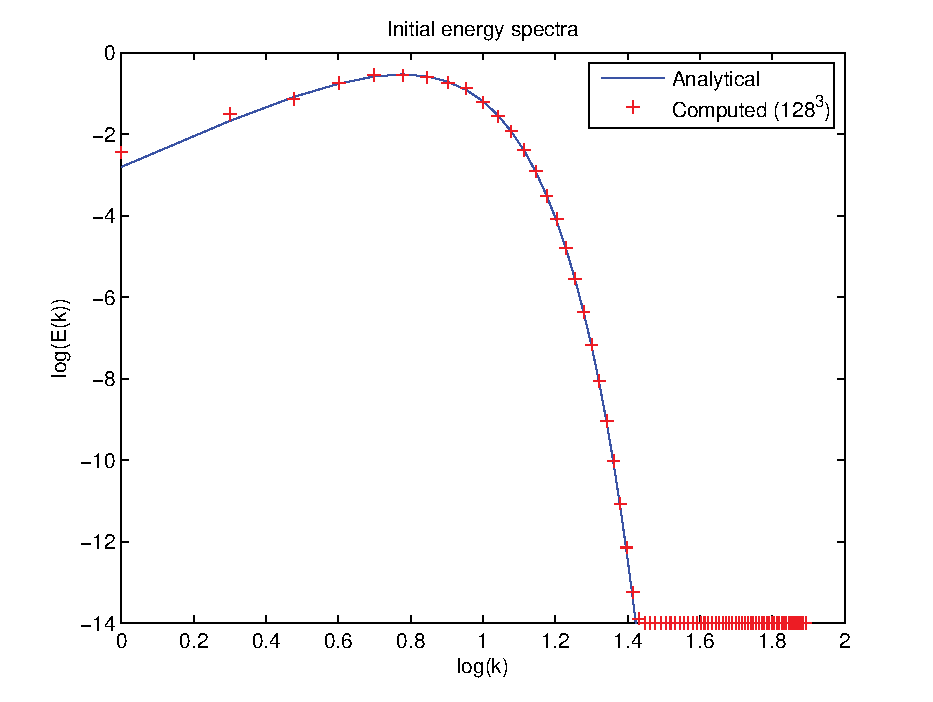
\includegraphics[width=0.6\textwidth]{Figures/Chapter3/DHIT_initial_energy}
	\caption{Analytical and computed initial energy spectrum for the DHIT test.}
	\label{fig-DHIT_initial_spectrum}
\end{figure}

In \Fig{DHIT_isovorticity} we depict the characteristic structures of a fully developed homogeneous and isotropic turbulent flow, plotting the vorticity isosurfaces obtained in the DHIT tes.
\begin{figure}[h!]
	\centering	
	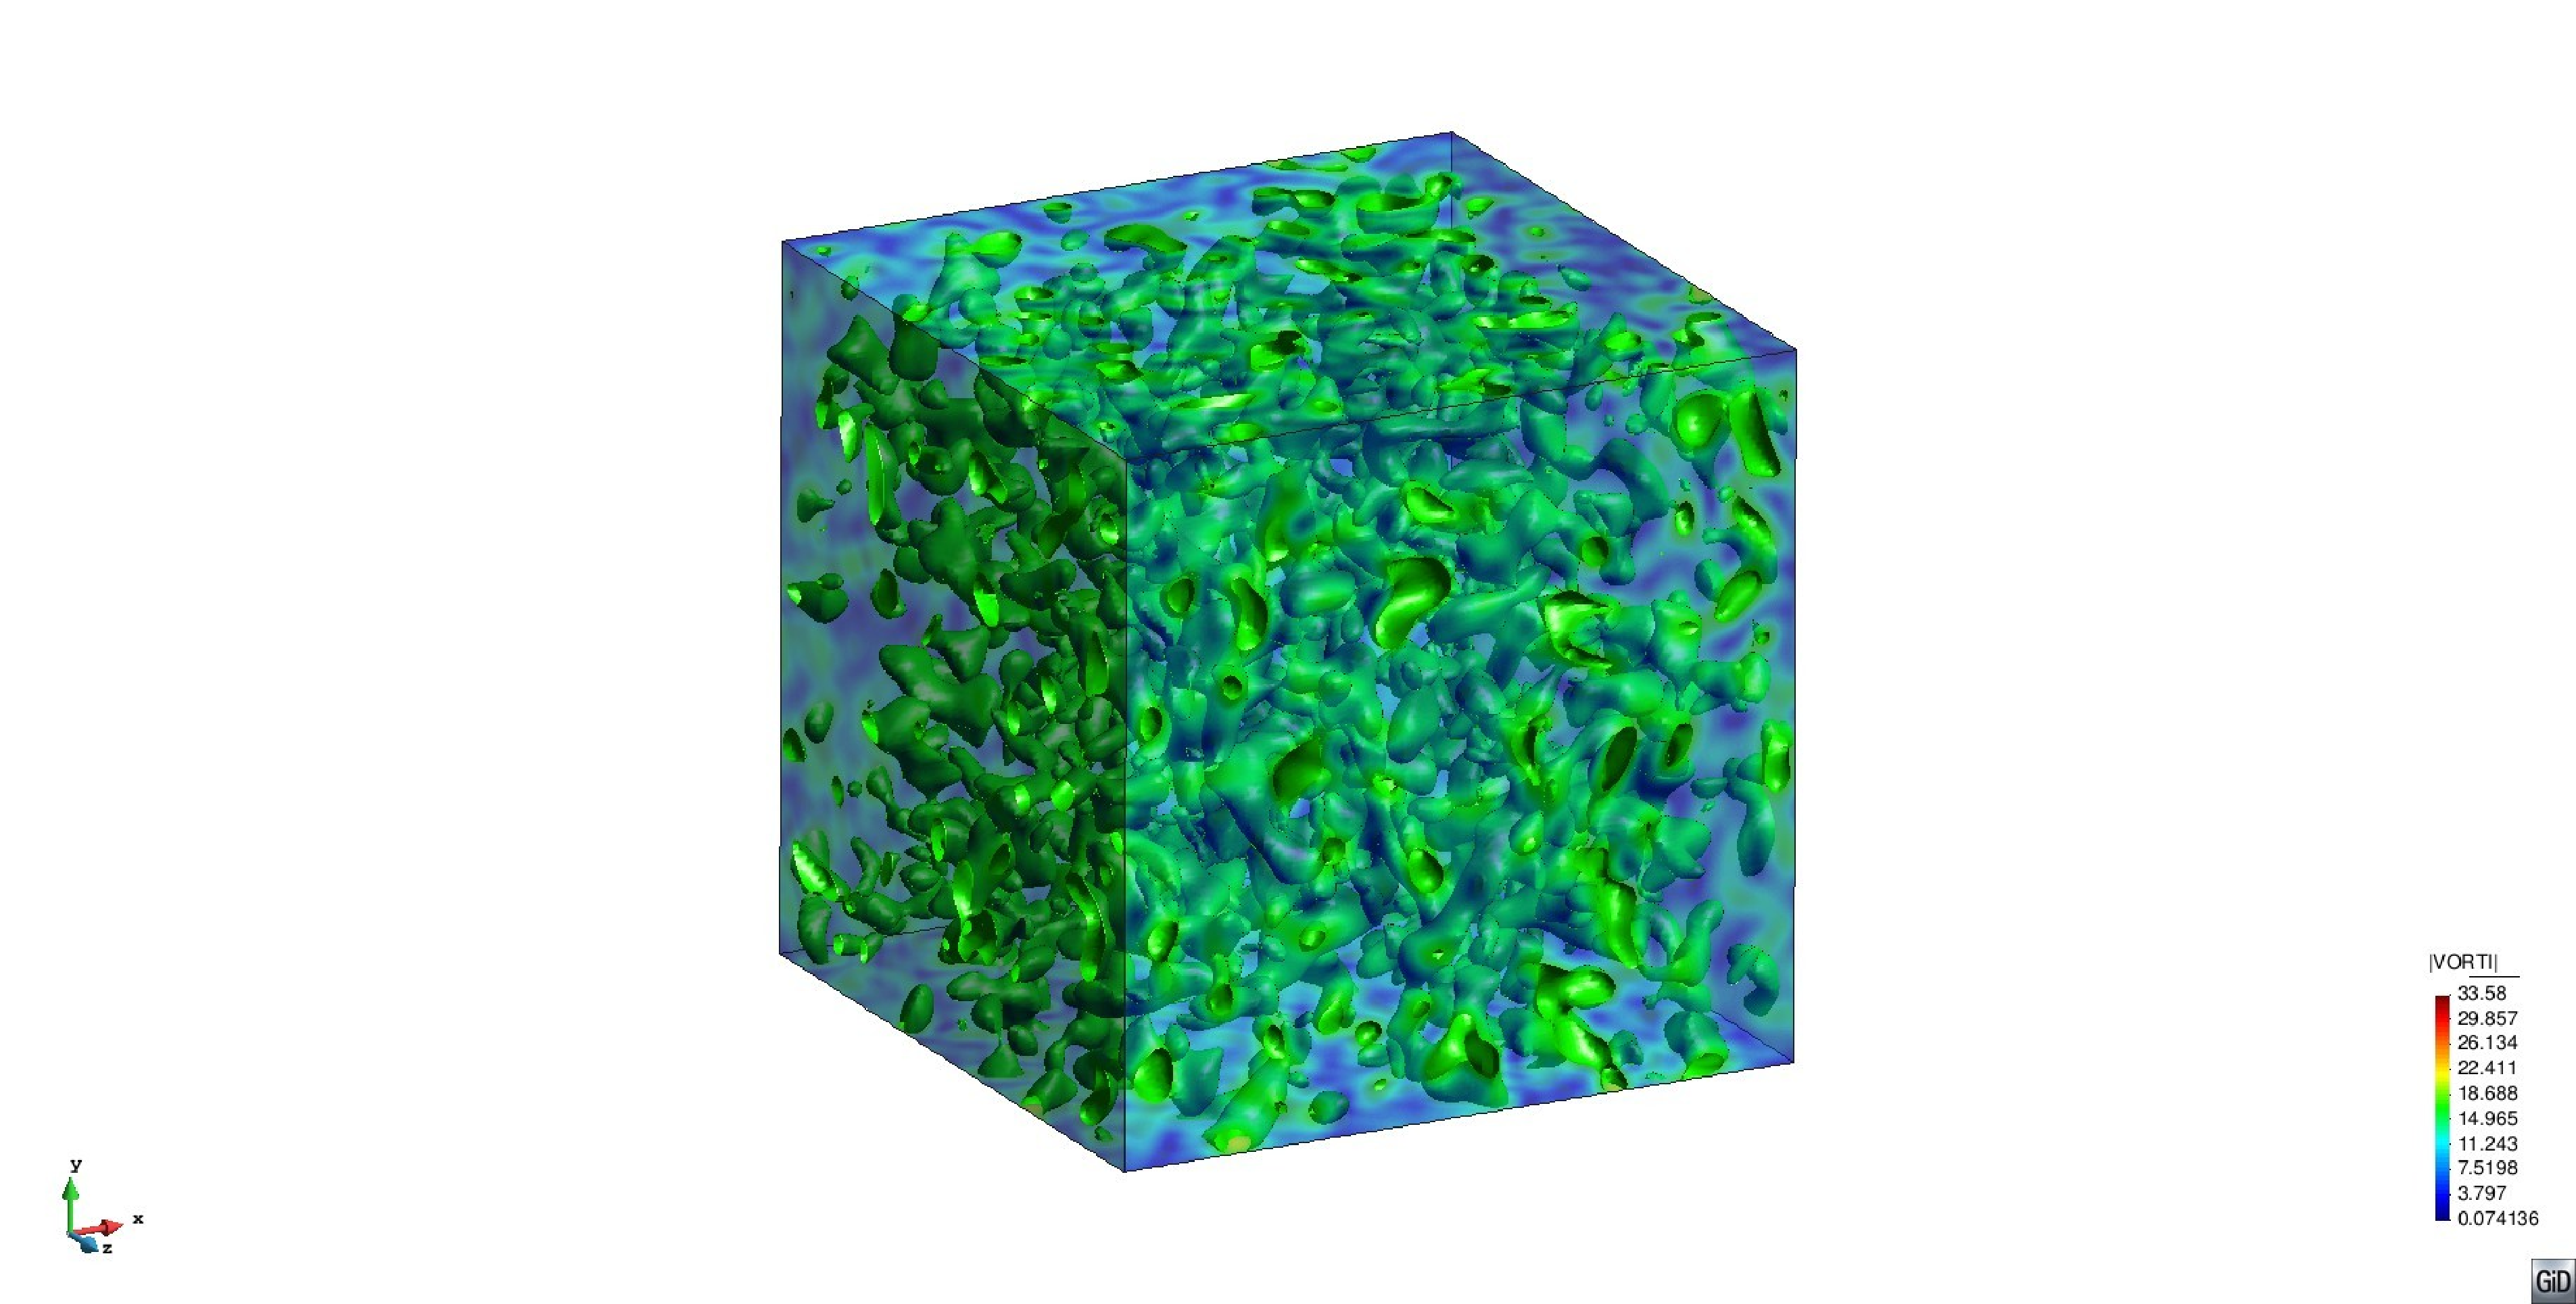
\includegraphics[trim=18cm 3.3cm 14cm 3.2cm,clip=true,width=0.7\textwidth]{Figures/Chapter3/DHIT_isovorticity}
	\caption{Vorticity isosurfaces in the DHIT test.}
	\label{fig-DHIT_isovorticity}
\end{figure}

The initial condition has a relevant role on homogeneous isotropic turbulence. In the final periods of decay, as has been exposed by \cite{hinze_turbulence_1975}, the energy spectrum follows the linear decay law,
\begin{equation}
\label{eq-DHIT_final_decay}
E(k,t)=E(k,0)\exp(-2\nu k^2t).
\end{equation}
So, a first conclusion we can point out from \Eq{DHIT_final_decay} is that the initial spectra, $E(k,0)$, in the final period of decay, has a direct relation with the decay exponent. The total kinetic energy can be calculated integrating \Eq{DHIT_final_decay} over all wave numbers. Then, when $t\rightarrow\infty$, the power law decay is determined by the shape of the initial spectrum.

Moreover, \cite{Staffman 1967} showed that if the initial field is generated by random impulsive forces, a spectrum of the form
\begin{equation}
\label{eq-DHIT_staffman_decay}
E(k,t)\sim k^2\exp(-2\nu k^2t)
\end{equation}
will ensue. Then, the total kinetic energy will decay with the law $K\sim t^{-3/2}$. But, anyway, we will not consider the case of having impulsive forces acting on the flow.

Also in this direction \cite{rohe_analysis_2010} and \cite{chalot_consistent_1998}, say that in the long-run, the energy should decay following the $t^{-1.4}$ law.

\subsubsection{Taylor-Green Vortex flow}
The Taylor-Green Vortex flow (TGV) problem is also a typical and widely used problem on turbulence numerical simulations. First introduced by Taylor and Green (1937) \cite{taylor}, this problem aims to show, in a relatively simple flow, the basic turbulence decay mechanisms like the turbulent energy cascade, the production of small eddies and the enhancement of dissipation by the stretching of vortex lines.

The initial analytical condition for this problem, unlike the DHIT problem, is defined on the physical space. Here we follow \cite{gassner_accuracy_????}, where the initial solution is defined by
\begin{align}
\label{eq-TGV_initial_condition}
&u_x=u_0\cos(x)\sin(y)\sin(z),\\\nonumber
&u_y=-u_0\sin(x)\cos(y)\sin(z),\\\nonumber
&u_z=0,\\\nonumber
&p=p_0+\frac{1}{16}\left(\cos(2x)+\cos(2y)\right)\left(\cos(2z)+2\right).
\end{align}
With
$$u_0=\frac{2}{\sqrt{3}}\sin\left(\gamma+\frac{2\pi}{3}\right).$$
We choose $\gamma=0$, which gives the mean initial velocity  $u_0=1$. The Reynolds number is defined as the inverse of the kinematic viscosity $\nu$, noting that the length and velocity scales are of the same order. This is done according to \cite{gassner_accuracy_????} and \cite{brachet_direct_1991}, and will allow us to compare our results with those showed on these papers. For simplicity, the pressure constant parameter $p_0$ is choosen equal to zero.

With these definitions we can compute analitycaly the initial total kinetic energy of the problem, which is 
\begin{align}
\label{eq-TGV_initial_energy}
K&=\frac{1}{2}\frac{1}{V}\int_0^L\int_0^L\int_0^L\u\cdot\u\ dV\\\nonumber
&=\frac{1}{16\pi^3}\int_0^{2\pi}\int_0^{2\pi}\int_0^{2\pi}\left(u_x^2+u_y^2+u_z^2\right)dxdydz\\\nonumber
&=\frac{u_0^2}{16\pi^3}\int_0^{2\pi}\int_0^{2\pi}\int_0^{2\pi}\left(\cos^2(x)\sin^2(y)+\sin^2(x)\cos^2(y)\right)\sin^2(z)dxdydz\\\nonumber
&=\frac{u_0^2}{8}.
\end{align}

We also can calculate the initial enstrophy of the problem, given by the following expression
\begin{align}
\label{eq-TGV_wnstrophy}
Z&=\frac{1}{2V}\int_0^L\int_0^L\int_0^L\nabla\u:\nabla\u\ dV\\\nonumber
&=\frac{1}{16\pi^3}\int_0^{2\pi}\int_0^{2\pi}\int_0^{2\pi}\left(\sum_{i=1}^3\sum_{j=1}^3\left(\frac{\partial u_i}{\partial x_j}\right)^2\right)dxdydz\\\nonumber
&=\frac{u_0^2}{16\pi^3}\int_0^{2\pi}\int_0^{2\pi}\int_0^{2\pi}\left[2\sin^2(z)\left(\sin^2(x)\sin^2(y)+\cos^2(x)\cos^2(y)\right)\right.\\\nonumber
&+\left.\cos^2(z)\left(\cos^2(x)\sin^2(y)+\sin^2(x)\cos^2(y)\right)\right]dxdydz\\\nonumber
&=\frac{3}{8}u_0^2.
\end{align}

Another interesting result coming from the definition of the initial condition \Eq{TGV_initial_condition} is its representation on the Fourier space. According to Fauconnier et al, \cite{fauconnier_construction_2009}, the initial velocity field on the Fourier space corresponds to eight Fourier modes located at $\mathbf{k}=(\pm1,\pm1,\pm1)$. It means that the initial flow generates a single  vortex scale.

One of the peculiarities about the TGV test is that the initial condition has two-dimensional streamlines, on the $x-y$ plan, but the flow is three dimensional (the initial velocity field also depends on the $z$ direction). 

It is also important to be said that the initial flow is highly symmetric. This symmetry makes that, as stressed by Brachet et al. \cite{brachet_small-scale_1983}, for all times, no fluid crosses any plan such that $x$, $y$ or $z=n\pi$, being $n$ an integer. Taking into account these flow properties we can define the region $0\leq x,y,z\leq\pi$ as the \textit{impermeable box}, since there is a confination of the flow inside this domain. The whole region, $0\leq x,y,z\leq2\pi$, can be called the \textit{periodic box}. Finally, due to the flow symmetries, there is a region from which we can determine the flow at any point in the space. This region is called \textit{fundamental box} and is generated by the box $0\leq x,y,z\leq\frac{1}{2}\pi$.

It can be seen that the perpendicular velocity component, $u_\perp$, and the normal derivative of the parallel velocity component, $\frac{\partial u_\parallel}{\partial n}$, for each impermeable box face vanish on this face. That is, given a face $\Gamma_i$
\begin{align}
\label{eq-TGV_u_perp}
u_\perp|_{\Gamma_i}=0,\quad\mbox{and}\quad\frac{\partial u_\parallel}{\partial n}|_{\Gamma_i}=0.
\end{align}

Equation \Eq{TGV_u_perp} has a direct implication to the voritcity field, $\boldsymbol{\omega}$. For a given impermeable box face, the vorticity on this face can be defined in terms of perpendicular and parallel components as
\begin{align}
\label{eq-TGV_vorticity}
\omega_{\parallel_1}=\left(\frac{\partial u_{\parallel_2}}{\partial x_\perp}-\frac{\partial u_\perp}{\partial x_{\parallel_2}}\right)=0,\\\nonumber
\omega_{\parallel_2}=\left(\frac{\partial u_{\parallel_1}}{\partial x_\perp}-\frac{\partial u_\perp}{\partial x_{\parallel_1}}\right)=0,\\\nonumber
\omega_\perp=\left(\frac{\partial u_{\parallel_1}}{\partial x_{\parallel_2}}-\frac{\partial u_{\parallel_2}}{\partial x_{\parallel_1}}\right)\neq0.
\end{align}
Which means that the vorticity is perpendicular to each impermeable box face.

We solve the Taylor-Green vortex (TG) problem using a Reynolds number $Re=1600$. The most common Reynolds numbers available in the literature are ${\rm Re}=800$, ${\rm Re}=1600$ and ${\rm Re}=3000$ (see, e.g., \cite{andrea_d._beck_numerical_2012, fauconnier_construction_2009, gassner_accuracy_????, jb_chapelier_final_2012}).

The TGV test is characterized by its laminar evolution at the initial time steps, when the flow is strongly anisotropic due to the structured large-scale vortexes directly related to the initial condition. If the Reynolds number is large enough, there appears the vortex-stretching process, which introduce the energy cascade effect, transfering energy from large to small-scales. Because of this procedure, the flow becomes unstable and, therefore, turbulent. According to Brachet et al. \cite{brachet_small-scale_1983}, the flow becomes nearly isotropic for $Re\geq1000$.

In \Fig{TGV_vorticity_streamlines} we depict a vorticity isosurface image computed using a $128^3$ trilinear hexaedral elements mesh. In this picture we can see the symmetry plans stated before.

%\begi\end{figure}d{figure}
\begin{figure}[h!]
	\centering	
	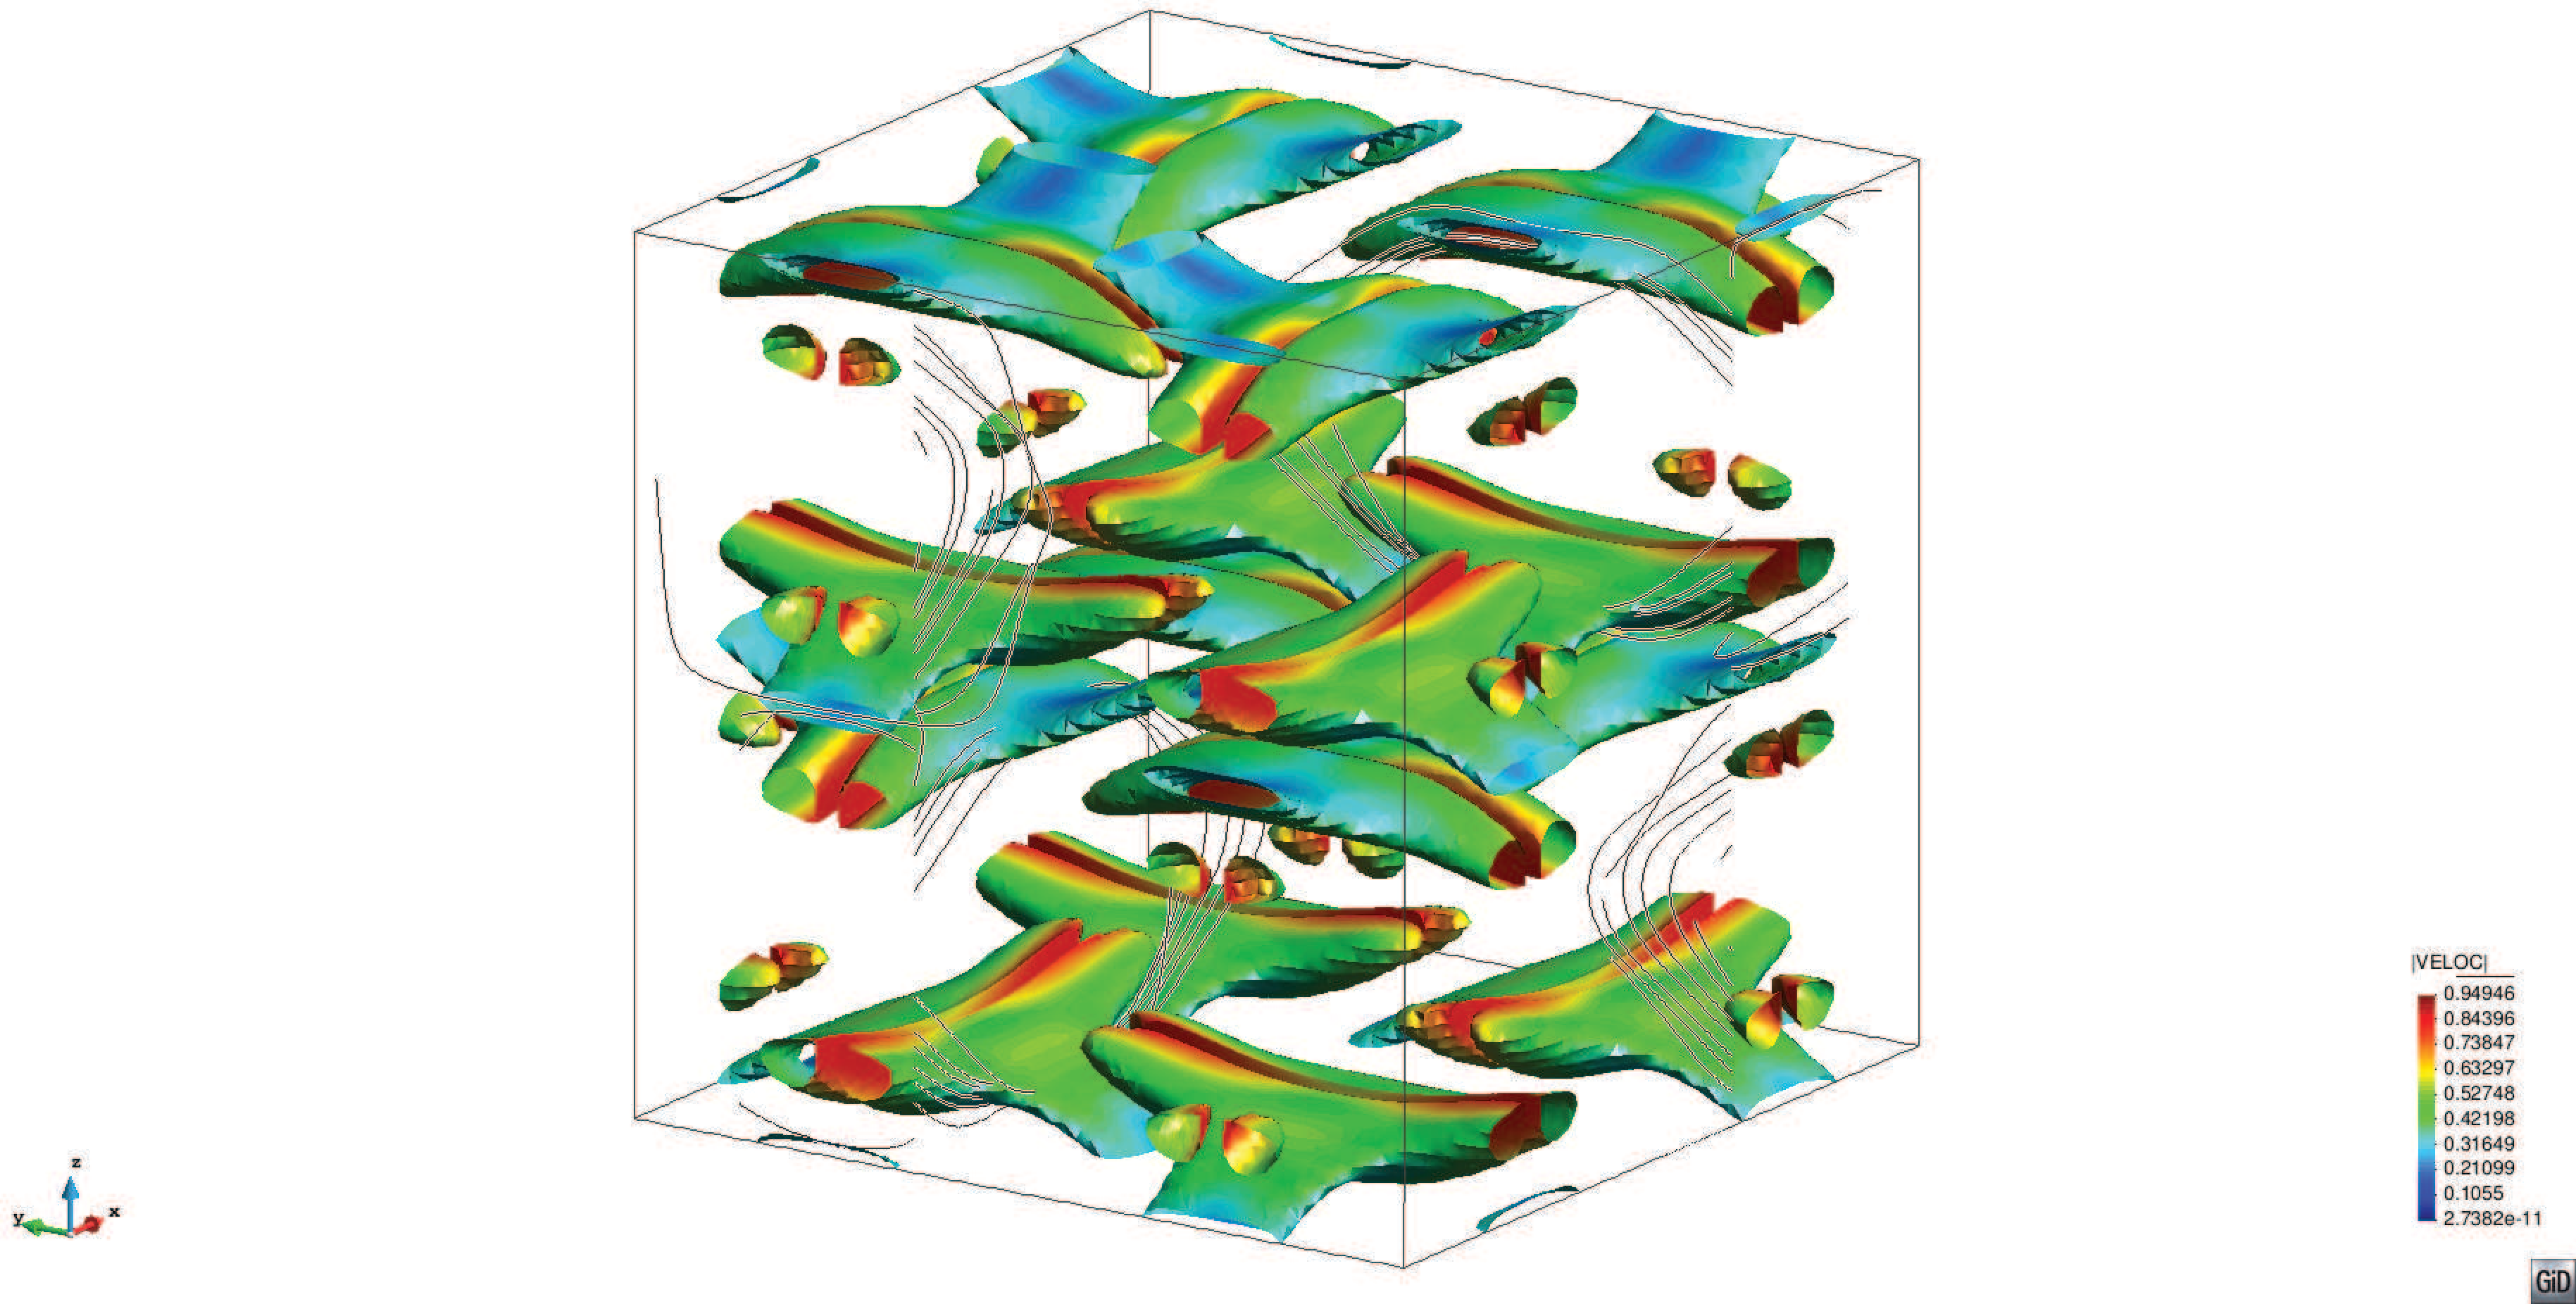
\includegraphics[clip=true, trim=13cm 0cm 13cm 0cm, width=0.6\textwidth]{Figures/Chapter3/TGV_isovorti_streaml_veloc_1}
	\caption{Vorticity isosurfaces at $t=4,0$ with streamlines for the TGV test.}
	\label{fig-TGV_vorticity_streamlines}
\end{figure}

\section{Turbulence in wall-bounded flow}
The vast majority of turbulent flows that we can find in the nature are bounded by, at least, one solid surface. Some examples of bounded flows can be the flow throug a pipe or a duct, the flow in a channel or a river, the flow around an aircraft or a ship, or even the atmospheric flow that is bounded by the terrain. In a turbulent wall-bounded flow, the turbulence is generated through the viscous forces near the wall and then propagated to the outer layer. In this kind of flows, we are interested on defining the mean velocity profiles as well as the friction laws, which will allow us to determine the forces that the fluid flow exerts on the the solid wall.
\subsection{Mean flow}
\subsubsection{Shear stress}
Let us assume that within a certain region near the wall the mean velocity is parallel, or almost parallel, to that wall. We consider that we have a wall on the plane $ (x-z) $ where the mean flow is predominantly in the $ x $-direction, which we will denote as the stream-wise direction and statistically independent of $ z $. The $ y $-direction will be denoted by the wall-normal direction and the $ z $-direction the span-wise direction. Under this assumtions, $ \left\langle u_z\right\rangle=0 $ and the $ \left\langle u_x\right\rangle $ is independent of $ x $, leading to a mean continuity equation
\begin{equation}
\label{eq-mean_continuity}
\frac{d\left\langle u_y\right\rangle}{dy}=0.
\end{equation}

From the mean meomentum equation in the wall-normal direction we can conclude that the pressure is uniform across the flow, satisfying $$ \frac{\partial\left\langle p\right\rangle}{\partial x}=\frac{d p_w}{dx}, $$ being $ p_w(x) $ the pressure value at the wall. Then, from the axial mean momentum equation we have that the shear total shear stress $ \tau(y) $ follows
\begin{equation}
\label{eq-shear_stress_law}
\frac{d\tau}{dy}=\frac{d p_w}{dx},
\end{equation}
with
\begin{equation}
\label{eq-shear_stress}
\tau(y):=\nu\frac{d\left\langle u_x\right\rangle}{dy}-\left\langle u_xu_y\right\rangle,
\end{equation}
see \cite{pope} for a more detailed deduction. We will denote the wall shear stress as $ \tau_w:=\tau(0) $. It is seen that the shear stress is the sum of the viscous stress, $ \nu\frac{d\left\langle u_x\right\rangle}{dy} $, and the Reynolds stress $ -\left\langle u_xu_y\right\rangle $. At the wall, the no-slip boundary condition, $ \u=0 $, implies that
\begin{equation}
\label{eq-wall_shear_stress}
\tau_w=\nu\left.\frac{d\left\langle u_x\right\rangle}{dy}\right|_{y=0}.
\end{equation}

\subsubsection{Friction quantities}
From \Eq{wall_shear_stress} one can observe that the viscosity $ \nu $ is an important parameter in tubulent wall-bounded flows, particularly in the region near the wall. Hence, the mean velocity profile  will depend on the Reynolds number. Moreover, in the region near the wall we can define the appropiate viscous velocity and length scales. We will call friction velocity the velocity scale in the near-wall region, which is defined as
\begin{equation}
\label{eq-friction_velocity}
u_\tau:=\sqrt{\frac{\tau_w}{\rho}},
\end{equation}
and the viscous length scale as 
\begin{equation}
\label{eq-viscous_lenghtscale}
\delta_\nu:=\nu\sqrt{\frac{\rho}{\tau_w}}=\frac{\nu}{u_\tau}.
\end{equation}
Note that the Reynolds number based on the viscous scales is equal to the unity, $ Re_\nu = \frac{u_\tau\delta_\nu}{\nu}=1 $. An alternative is the so called friction Reynolds number, which is defined as
\begin{equation}
\label{eq-friction_reynolds}
Re_\tau:=\frac{u_\tau\delta}{\nu},
\end{equation}
being $ \delta $ the boundary layer thicknes. 

For wall-bounded turbulent flows it is a common practise to use the quantities in terms of wall units. We will define the distance from the wall in wall units as $ y^+:=\frac{y}{\delta_\nu}=\frac{u_\tau y}{\nu} $, and the mean stream-wise velocity in wall units as $ u^+:=\frac{\left\langle u_x\right\rangle}{u_\tau} $.

\subsubsection{Velocity profile}
It has been shown that in the region near the wall, the mean stream-wise velocity can be defined by the distance to the wall. This is known as the law of the wall, which can be expressed in wall units as $ u^+=f_w(y^+) $. In the inner layer, where $ y/\delta\le0.1 $, the law of the wall has been shown to follow the following expression
\begin{equation}
\label{eq-wall_law}
u^+=\frac{1}{\kappa}\ln y^++B,
\end{equation}
whith $ \kappa=0.41 $ and $ B=5.2 $.

\subsection{Turbulent tests}
\subsubsection{Turbulent Channel Flow}
\subsubsection{Turbulent Flow around an airfoil}

\section{Outline and conclusions}

blablabla...

% Chapter 1

\chapter{Chapter Title Here} % Main chapter title

\label{Chapter1} % For referencing the chapter elsewhere, use \ref{Chapter1} 

%----------------------------------------------------------------------------------------

% Define some commands to keep the formatting separated from the content 
%\newcommand{\keyword}[1]{\textbf{#1}}
%\newcommand{\tabhead}[1]{\textbf{#1}}
%\newcommand{\code}[1]{\texttt{#1}}
%\newcommand{\file}[1]{\texttt{\bfseries#1}}
%\newcommand{\option}[1]{\texttt{\itshape#1}}

%----------------------------------------------------------------------------------------

\section{Welcome and Thank You}
Welcome to this \LaTeX{} Thesis Template, a beautiful and easy to use template for writing a thesis using the \LaTeX{} typesetting system.

If you are writing a thesis (or will be in the future) and its subject is technical or mathematical (though it doesn't have to be), then creating it in \LaTeX{} is highly recommended as a way to make sure you can just get down to the essential writing without having to worry over formatting or wasting time arguing with your word processor.

\LaTeX{} is easily able to professionally typeset documents that run to hundreds or thousands of pages long. With simple mark-up commands, it automatically sets out the table of contents, margins, page headers and footers and keeps the formatting consistent and beautiful. One of its main strengths is the way it can easily typeset mathematics, even \emph{heavy} mathematics. Even if those equations are the most horribly twisted and most difficult mathematical problems that can only be solved on a super-computer, you can at least count on \LaTeX{} to make them look stunning.

%----------------------------------------------------------------------------------------

\section{Learning \LaTeX{}}

\LaTeX{} is not a \textsc{wysiwyg} (What You See is What You Get) program, unlike word processors such as Microsoft Word or Apple's Pages. Instead, a document written for \LaTeX{} is actually a simple, plain text file that contains \emph{no formatting}. You tell \LaTeX{} how you want the formatting in the finished document by writing in simple commands amongst the text, for example, if I want to use \emph{italic text for emphasis}, I write the \verb|\emph{text}| command and put the text I want in italics in between the curly braces. This means that \LaTeX{} is a \enquote{mark-up} language, very much like HTML.

\subsection{A (not so short) Introduction to \LaTeX{}}

If you are new to \LaTeX{}, there is a very good eBook -- freely available online as a PDF file -- called, \enquote{The Not So Short Introduction to \LaTeX{}}. The book's title is typically shortened to just \emph{lshort}. You can download the latest version (as it is occasionally updated) from here:
\url{http://www.ctan.org/tex-archive/info/lshort/english/lshort.pdf}

It is also available in several other languages. Find yours from the list on this page: \url{http://www.ctan.org/tex-archive/info/lshort/}

It is recommended to take a little time out to learn how to use \LaTeX{} by creating several, small `test' documents, or having a close look at several templates on:\\ 
\url{http://www.LaTeXTemplates.com}\\ 
Making the effort now means you're not stuck learning the system when what you \emph{really} need to be doing is writing your thesis.

\subsection{A Short Math Guide for \LaTeX{}}

If you are writing a technical or mathematical thesis, then you may want to read the document by the AMS (American Mathematical Society) called, \enquote{A Short Math Guide for \LaTeX{}}. It can be found online here:
\url{http://www.ams.org/tex/amslatex.html}
under the \enquote{Additional Documentation} section towards the bottom of the page.

\subsection{Common \LaTeX{} Math Symbols}
There are a multitude of mathematical symbols available for \LaTeX{} and it would take a great effort to learn the commands for them all. The most common ones you are likely to use are shown on this page:
\url{http://www.sunilpatel.co.uk/latex-type/latex-math-symbols/}

You can use this page as a reference or crib sheet, the symbols are rendered as large, high quality images so you can quickly find the \LaTeX{} command for the symbol you need.

\subsection{\LaTeX{} on a Mac}
 
The \LaTeX{} distribution is available for many systems including Windows, Linux and Mac OS X. The package for OS X is called MacTeX and it contains all the applications you need -- bundled together and pre-customised -- for a fully working \LaTeX{} environment and workflow.
 
MacTeX includes a custom dedicated \LaTeX{} editor called TeXShop for writing your `\file{.tex}' files and BibDesk: a program to manage your references and create your bibliography section just as easily as managing songs and creating playlists in iTunes.

%----------------------------------------------------------------------------------------

\section{Getting Started with this Template}

If you are familiar with \LaTeX{}, then you should explore the directory structure of the template and then proceed to place your own information into the \emph{THESIS INFORMATION} block of the \file{main.tex} file. You can then modify the rest of this file to your unique specifications based on your degree/university. Section \ref{FillingFile} on page \pageref{FillingFile} will help you do this. Make sure you also read section \ref{ThesisConventions} about thesis conventions to get the most out of this template.

If you are new to \LaTeX{} it is recommended that you carry on reading through the rest of the information in this document.

Before you begin using this template you should ensure that its style complies with the thesis style guidelines imposed by your institution. In most cases this template style and layout will be suitable. If it is not, it may only require a small change to bring the template in line with your institution's recommendations. These modifications will need to be done on the \file{MastersDoctoralThesis.cls} file.

\subsection{About this Template}

This \LaTeX{} Thesis Template is originally based and created around a \LaTeX{} style file created by Steve R.\ Gunn from the University of Southampton (UK), department of Electronics and Computer Science. You can find his original thesis style file at his site, here:
\url{http://www.ecs.soton.ac.uk/~srg/softwaretools/document/templates/}

Steve's \file{ecsthesis.cls} was then taken by Sunil Patel who modified it by creating a skeleton framework and folder structure to place the thesis files in. The resulting template can be found on Sunil's site here:
\url{http://www.sunilpatel.co.uk/thesis-template}

Sunil's template was made available through \url{http://www.LaTeXTemplates.com} where it was modified many times based on user requests and questions. Version 2.0 and onwards of this template represents a major modification to Sunil's template and is, in fact, hardly recognisable. The work to make version 2.0 possible was carried out by \href{mailto:vel@latextemplates.com}{Vel} and Johannes Böttcher.

%----------------------------------------------------------------------------------------

\section{What this Template Includes}

\subsection{Folders}

This template comes as a single zip file that expands out to several files and folders. The folder names are mostly self-explanatory:

\keyword{Appendices} -- this is the folder where you put the appendices. Each appendix should go into its own separate \file{.tex} file. An example and template are included in the directory.

\keyword{Chapters} -- this is the folder where you put the thesis chapters. A thesis usually has about six chapters, though there is no hard rule on this. Each chapter should go in its own separate \file{.tex} file and they can be split as:
\begin{itemize}
\item Chapter 1: Introduction to the thesis topic
\item Chapter 2: Background information and theory
\item Chapter 3: (Laboratory) experimental setup
\item Chapter 4: Details of experiment 1
\item Chapter 5: Details of experiment 2
\item Chapter 6: Discussion of the experimental results
\item Chapter 7: Conclusion and future directions
\end{itemize}
This chapter layout is specialised for the experimental sciences.

\keyword{Figures} -- this folder contains all figures for the thesis. These are the final images that will go into the thesis document.

\subsection{Files}

Included are also several files, most of them are plain text and you can see their contents in a text editor. After initial compilation, you will see that more auxiliary files are created by \LaTeX{} or BibTeX and which you don't need to delete or worry about:

\keyword{example.bib} -- this is an important file that contains all the bibliographic information and references that you will be citing in the thesis for use with BibTeX. You can write it manually, but there are reference manager programs available that will create and manage it for you. Bibliographies in \LaTeX{} are a large subject and you may need to read about BibTeX before starting with this. Many modern reference managers will allow you to export your references in BibTeX format which greatly eases the amount of work you have to do.

\keyword{MastersDoctoralThesis.cls} -- this is an important file. It is the class file that tells \LaTeX{} how to format the thesis. If you need to change the layout or structure of the thesis, you will likely need to open this file and find the part relevant to what you are trying to do.

\keyword{main.pdf} -- this is your beautifully typeset thesis (in the PDF file format) created by \LaTeX{}. It is supplied in the PDF with the template and after you compile the template you should get an identical version.

\keyword{main.tex} -- this is an important file. This is the file that you tell \LaTeX{} to compile to produce your thesis as a PDF file. It contains the framework and constructs that tell \LaTeX{} how to layout the thesis. It is heavily commented so you can read exactly what each line of code does and why it is there. After you put your own information into the \emph{THESIS INFORMATION} block -- you have now started your thesis!

Files that are \emph{not} included, but are created by \LaTeX{} as auxiliary files include:

\keyword{main.aux} -- this is an auxiliary file generated by \LaTeX{}, if it is deleted \LaTeX{} simply regenerates it when you run the main \file{.tex} file.

\keyword{main.bbl} -- this is an auxiliary file generated by BibTeX, if it is deleted, BibTeX simply regenerates it when you run the `main' file. Whereas the \file{.bib} file contains all the references you have, this \file{.bbl} file contains the references you have actually cited in the thesis and is used to build the bibliography section of the thesis.

\keyword{main.blg} -- this is an auxiliary file generated by BibTeX, if it is deleted BibTeX simply regenerates it when you run the main \file{.tex} file.

\keyword{main.lof} -- this is an auxiliary file generated by \LaTeX{}, if it is deleted \LaTeX{} simply regenerates it when you run the main \file{.tex} file. It tells \LaTeX{} how to build the \emph{List of Figures} section.

\keyword{main.log} -- this is an auxiliary file generated by \LaTeX{}, if it is deleted \LaTeX{} simply regenerates it when you run the main \file{.tex} file. It contains messages from \LaTeX{}, if you receive errors and warnings from \LaTeX{}, they will be in this \file{.log} file.

\keyword{main.lot} -- this is an auxiliary file generated by \LaTeX{}, if it is deleted \LaTeX{} simply regenerates it when you run the main \file{.tex} file. It tells \LaTeX{} how to build the \emph{List of Tables} section.

\keyword{main.out} -- this is an auxiliary file generated by \LaTeX{}, if it is deleted \LaTeX{} simply regenerates it when you run the main \file{.tex} file.

So from this long list, only the files with the \file{.bib}, \file{.cls} and \file{.tex} extensions are the most important ones. The other auxiliary files can be ignored or deleted as \LaTeX{} and BibTeX will regenerate them.

%----------------------------------------------------------------------------------------

\section{Filling in Your Information in the \file{main.tex} File}\label{FillingFile}

You will need to personalise the thesis template and make it your own by filling in your own information. This is done by editing the \file{main.tex} file in a text editor.

Open the file and scroll down to the second large block titled \emph{THESIS INFORMATION} where you can see the entries for \emph{University Name}, \emph{Department Name}, etc \ldots

Fill out the information about yourself, your group and institution. You can also insert web links, if you do, make sure you use the full URL, including the \code{http://} for this. If you don't want these to be linked, simply remove the \verb|\href{url}{name}| and only leave the name.

When you have done this, save the file and recompile \code{main.tex}. All the information you filled in should now be in the PDF, complete with web links. You can now begin your thesis proper!

%----------------------------------------------------------------------------------------

\section{The \code{main.tex} File Explained}

The \file{main.tex} file contains the structure of the thesis. There are plenty of written comments that explain what pages, sections and formatting the \LaTeX{} code is creating. Each major document element is divided into commented blocks with titles in all capitals to make it obvious what the following bit of code is doing. Initially there seems to be a lot of \LaTeX{} code, but this is all formatting, and it has all been taken care of so you don't have to do it.

Begin by checking that your information on the title page is correct. For the thesis declaration, your institution may insist on something different than the text given. If this is the case, just replace what you see with what is required in the \emph{DECLARATION PAGE} block.

Then comes a page which contains a funny quote. You can put your own, or quote your favourite scientist, author, person, and so on. Make sure to put the name of the person who you took the quote from.

Following this is the abstract page which summaries your work in a condensed way and can almost be used as a standalone document to describe what you have done. The text you write will cause the heading to move up so don't worry about running out of space.

Next come the acknowledgements. On this page, write about all the people who you wish to thank (not forgetting parents, partners and your advisor/supervisor).

The contents pages, list of figures and tables are all taken care of for you and do not need to be manually created or edited. The next set of pages are more likely to be optional and can be deleted since they are for a more technical thesis: insert a list of abbreviations you have used in the thesis, then a list of the physical constants and numbers you refer to and finally, a list of mathematical symbols used in any formulae. Making the effort to fill these tables means the reader has a one-stop place to refer to instead of searching the internet and references to try and find out what you meant by certain abbreviations or symbols.

The list of symbols is split into the Roman and Greek alphabets. Whereas the abbreviations and symbols ought to be listed in alphabetical order (and this is \emph{not} done automatically for you) the list of physical constants should be grouped into similar themes.

The next page contains a one line dedication. Who will you dedicate your thesis to?

Finally, there is the block where the chapters are included. Uncomment the lines (delete the \code{\%} character) as you write the chapters. Each chapter should be written in its own file and put into the \emph{Chapters} folder and named \file{Chapter1}, \file{Chapter2}, etc\ldots Similarly for the appendices, uncomment the lines as you need them. Each appendix should go into its own file and placed in the \emph{Appendices} folder.

After the preamble, chapters and appendices finally comes the bibliography. The bibliography style (called \option{authoryear}) is used for the bibliography and is a fully featured style that will even include links to where the referenced paper can be found online. Do not underestimate how grateful your reader will be to find that a reference to a paper is just a click away. Of course, this relies on you putting the URL information into the BibTeX file in the first place.

%----------------------------------------------------------------------------------------

\section{Thesis Features and Conventions}\label{ThesisConventions}

To get the best out of this template, there are a few conventions that you may want to follow.

One of the most important (and most difficult) things to keep track of in such a long document as a thesis is consistency. Using certain conventions and ways of doing things (such as using a Todo list) makes the job easier. Of course, all of these are optional and you can adopt your own method.

\subsection{Printing Format}

This thesis template is designed for double sided printing (i.e. content on the front and back of pages) as most theses are printed and bound this way. This means that the inner margin is always wider than the outer for binding. Four out of five people will now judge the margins by eye and think, \enquote{I never noticed that before}. Switching to one sided printing is as simple as uncommenting the \option{oneside} option of the \code{documentclass} command at the top of the \file{main.tex} file. You may then wish to adjust the margins to suit specifications from your institution.

The headers for the pages contain the page number on the outer side (so it is easy to flick through to the page you want) and the chapter name on the inner side.

The text is set to 11 point by default with single line spacing, again, you can tune the text size and spacing should you want or need to using the options at the very start of \file{main.tex}. The spacing can be changed similarly by replacing the \option{singlespacing} with \option{onehalfspacing} or \option{doublespacing}.

\subsection{Using US Letter Paper}

The paper size used in the template is A4, which is the standard size in Europe. If you are using this thesis template elsewhere and particularly in the United States, then you may have to change the A4 paper size to the US Letter size. To do this, you will need to open the \file{MastersDoctoralThesis.cls} file and navigate to the \code{MARGINS} block where you can change \option{a4paper} to \option{letterpaper}.

Due to the differences in the paper size, the resulting margins may be different to what you like or require (as it is common for institutions to dictate certain margin sizes). If this is the case, then the margin sizes can be tweaked by modifying the values in the same block as where you set the paper size. Now your document should be set up for US Letter paper size with suitable margins.

\subsection{References}

The \code{biblatex} package is used to format the bibliography and inserts references such as this one \parencite{Reference1}. The options used in the \file{main.tex} file mean that the in-text citations of references are formatted with the author(s) listed with the date of the publication. Multiple references are separated by semicolons (e.g. \parencite{Reference2, Reference1}) and references with more than three authors are only show the first author with \emph{et al.} indicating there are more authors (e.g. \parencite{Reference3}). This is done automatically for you. To see how you use references, have a look at the \file{Chapter1.tex} source file. Many reference managers allow you to simply drag the reference into the document as you type.

Scientific references should come \emph{before} the punctuation mark if there is one (such as a comma or period). The same goes for footnotes\footnote{Such as this footnote, here down at the bottom of the page.}. You can change this but the most important thing is to keep the convention consistent throughout the thesis. Footnotes themselves should be full, descriptive sentences (beginning with a capital letter and ending with a full stop). The APA6 states: ``Footnote numbers should be superscripted, [...], following any punctuation mark except a dash.'' The Chicago manual of style states: ``A note number should be placed at the end of a sentence or clause. The number follows any punctuation mark except the dash, which it precedes. It follows a closing parenthesis.''

The bibliography is typeset with references listed in alphabetical order by the first author's last name. This is similar to the APA referencing style. To see how \LaTeX{} typesets the bibliography, have a look at the very end of this document (or just click on the reference number links in in-text citations).

\subsubsection{A Note on bibtex}

The bibtex backend used in the template by default does not correctly handle unicode character encoding (i.e. "international" characters). You may see a warning about this in the compilation log and, if your references contain unicode characters, they may not show up correctly or at all. The solution to this is to use the biber backend instead of the outdated bibtex backend. This is done by finding this in \file{main.tex}: \option{backend=bibtex} and changing it to \option{backend=biber}. You will then need to delete all auxiliary BibTeX files and navigate to the template directory in your terminal (command prompt). Once there, simply type \code{biber main} and biber will compile your bibliography. You can then compile \file{main.tex} as normal and your bibliography will be updated. An alternative is to set up your LaTeX editor to compile with biber instead of bibtex, see \href{http://tex.stackexchange.com/questions/154751/biblatex-with-biber-configuring-my-editor-to-avoid-undefined-citations/}{here} for how to do this for various editors.

\subsection{Tables}

Tables are an important way of displaying your results, below is an example table which was generated with this code:

{\small
\begin{verbatim}
\begin{table}
\caption{The effects of treatments X and Y on the four groups studied.}
\label{tab:treatments}
\centering
\begin{tabular}{l l l}
\toprule
\tabhead{Groups} & \tabhead{Treatment X} & \tabhead{Treatment Y} \\
\midrule
1 & 0.2 & 0.8\\
2 & 0.17 & 0.7\\
3 & 0.24 & 0.75\\
4 & 0.68 & 0.3\\
\bottomrule\\
\end{tabular}
\end{table}
\end{verbatim}
}

\begin{table}
\caption{The effects of treatments X and Y on the four groups studied.}
\label{tab:treatments}
\centering
\begin{tabular}{l l l}
\toprule
\tabhead{Groups} & \tabhead{Treatment X} & \tabhead{Treatment Y} \\
\midrule
1 & 0.2 & 0.8\\
2 & 0.17 & 0.7\\
3 & 0.24 & 0.75\\
4 & 0.68 & 0.3\\
\bottomrule\\
\end{tabular}
\end{table}

You can reference tables with \verb|\ref{<label>}| where the label is defined within the table environment. See \file{Chapter1.tex} for an example of the label and citation (e.g. Table~\ref{tab:treatments}).

\subsection{Figures}

There will hopefully be many figures in your thesis (that should be placed in the \emph{Figures} folder). The way to insert figures into your thesis is to use a code template like this:
\begin{verbatim}
\begin{figure}
\centering

\includegraphics{./Figures/Electron}
\decoRule
\caption[An Electron]{An electron (artist's impression).}
\label{fig:Electron}
\end{figure}
\end{verbatim}
Also look in the source file. Putting this code into the source file produces the picture of the electron that you can see in the figure below.

\begin{figure}[h]
\centering
%
\includegraphics{../Figures/Electron.pdf}
\decoRule
\caption[An Electron]{An electron (artist's impression).}
\label{fig:Electron}
\end{figure}

Sometimes figures don't always appear where you write them in the source. The placement depends on how much space there is on the page for the figure. Sometimes there is not enough room to fit a figure directly where it should go (in relation to the text) and so \LaTeX{} puts it at the top of the next page. Positioning figures is the job of \LaTeX{} and so you should only worry about making them look good!

Figures usually should have captions just in case you need to refer to them (such as in Figure~\ref{fig:Electron}). The \verb|\caption| command contains two parts, the first part, inside the square brackets is the title that will appear in the \emph{List of Figures}, and so should be short. The second part in the curly brackets should contain the longer and more descriptive caption text.

The \verb|\decoRule| command is optional and simply puts an aesthetic horizontal line below the image. If you do this for one image, do it for all of them.

\LaTeX{} is capable of using images in many formats such as PDF, JPEG, PNG and more.

\subsection{Typesetting mathematics}

If your thesis is going to contain heavy mathematical content, be sure that \LaTeX{} will make it look beautiful, even though it won't be able to solve the equations for you.

The \enquote{Not So Short Introduction to \LaTeX} (available on \href{http://www.ctan.org/tex-archive/info/lshort/english/lshort.pdf}{CTAN}) should tell you everything you need to know for most cases of typesetting mathematics. If you need more information, a much more thorough mathematical guide is available from the AMS called, \enquote{A Short Math Guide to \LaTeX} and can be downloaded from:
\url{ftp://ftp.ams.org/pub/tex/doc/amsmath/short-math-guide.pdf}

There are many different \LaTeX{} symbols to remember, luckily you can find the most common symbols \href{http://www.sunilpatel.co.uk/latexsymbols.html}{here}. You can use the web page as a quick reference or crib sheet and because the symbols are grouped and rendered as high quality images (each with a downloadable PDF), finding the symbol you need is quick and easy.

You can write an equation, which is automatically given an equation number by \LaTeX{} like this:
\begin{verbatim}
\begin{equation}
E = mc^{2}
\label{eqn:Einstein}
\end{equation}
\end{verbatim}

This will produce Einstein's famous energy-matter equivalence equation:
\begin{equation}
E = mc^{2}
\label{eqn:Einstein}
\end{equation}

All equations you write (which are not in the middle of paragraph text) are automatically given equation numbers by \LaTeX{}. If you don't want a particular equation numbered, use the unnumbered form:
\begin{verbatim}
\[ a^{2}=4 \]
\end{verbatim}

%----------------------------------------------------------------------------------------

\section{Sectioning and Subsectioning}

You should break your thesis up into nice, bite-sized sections and subsections. \LaTeX{} automatically builds a table of Contents by looking at all the \verb|\chapter{}|, \verb|\section{}|  and \verb|\subsection{}| commands you write in the source.

The Table of Contents should only list the sections to three (3) levels. A \verb|chapter{}| is level zero (0). A \verb|\section{}| is level one (1) and so a \verb|\subsection{}| is level two (2). In your thesis it is likely that you will even use a \verb|subsubsection{}|, which is level three (3). The depth to which the Table of Contents is formatted is set within \file{MastersDoctoralThesis.cls}.

%----------------------------------------------------------------------------------------

\section{In Closing}

You have reached the end of this mini-guide. You can now rename or overwrite this pdf file and begin writing your own \file{Chapter1.tex}' and the rest of your thesis. The easy work of setting up the structure and framework has been taken care of for you. It's now your job to fill it out!

Good luck and have lots of fun!

\begin{flushright}
Guide written by ---\\
Sunil Patel: \href{http://www.sunilpatel.co.uk}{www.sunilpatel.co.uk}\\
Vel: \href{http://www.LaTeXTemplates.com}{LaTeXTemplates.com}
\end{flushright}
 

%----------------------------------------------------------------------------------------
%	THESIS CONTENT - APPENDICES
%----------------------------------------------------------------------------------------

\appendix % Cue to tell LaTeX that the following "chapters" are Appendices

% Include the appendices of the thesis as separate files from the Appendices folder
% Uncomment the lines as you write the Appendices

% Appendix A

\chapter{Energy spectrum computation} % Main appendix title
\label{appendix-spectrum_implementation}

\label{apenA-energy_spectrum_implementation} % For referencing this appendix elsewhere, use \ref{AppendixA}

In this appendix we will briefly resume the code that has to be implemented to obtain the energy spectra of a turbulent fluid sample.

We assume that we are working with a two-dimensional fluid flow with periodic boundary conditions on both directions. We also assume that we compute the energy spectrum from the velocity field, comming from the Navier-Stoke equations. There also are many works on the turbulence world that use the vorticity field to calculate the energy spectra.

As we are using a Finite Element Method to calculate the velocity field, our data will be a discrete data with the values of the velocity on each node of the FEM mesh. The first thing we need to do is to store the velocity field into an array with the same components as problem dimensions. Usually, the velocity field that arise after the solution of the FE system of equations is stored in a vector. Then, we must transform the velocity field into two-dimensional array, having a matrix with the same rows as nodes in the vertical direction and the same columns as nodes in the horitzontal direction. The matrix values must be stored in the equivalent position than the node position in the FEM mesh.

It also has to be said that for a problem with periodic boundary conditions we only have to transform those values that are not repeated. For a two-dimensional grid with $N_x\times N_y$ divisions ($(N_x+1)\times(N_y+1)$ nodes), the values to be transformed are those corresponding to the nodes $1$ to $N_x$, in the $x$-direction, and $1$ to $N_y$, in the $y$-direction. The $(N_x+1)$-th and $(N_y+1)$-th nodes have the same value as the first ones.

Once we have obtained the velocity field and we have transformed into a two dimensional array, we follow the following steps.

\begin{itemize}
\item[1.]\textit{FFT transform of the velocity field}

At this point we perform the Discrete Fast Fourier Transform (DFFT) of each component of the velocity field. To do that we use the \textit{fft99} and \textit{cfft99} packages that we can find in \cite{orlandi}. The first code transforms a real data vector to a half-complex vector with the transformed field. The second one transforms a complex vector to another complex vector with the transformed field.

Both packages are based on the following Discrete Fast Fourier Transform definitions:
\begin{equation*}
\label{1.12.1}
f_k=\sum_{n=0}^{N-1}f_ne^{-i\frac{2\pi kn}{N}},\quad\quad\mbox{(Forward transform)}
\end{equation*}
\begin{equation*}
\label{1.12.2}
f_n=\sum_{k=0}^{N-1}f_ke^{i\frac{2\pi kn}{N}},\quad\quad\mbox{(Backward transform)}
\end{equation*}
with $k$ the wave number, $N$ the number of values to transform, $f_k$ the $k$-th value of the transformed vector and $f_n$ the $n$-th value of the original vector.

We also must have into account that to use these packages the lengths of the transforms must be an even number greater than 4 that has no other prime factors than 2, 3 and 5.

Since we have a two-dimensional real data field, and using the Fourier Transforms theory, we compute the two-dimensional transform by first transforming a set of vectors using \textit{fft99} along one direction and then transforming the results using \textit{cfft99} along the orthogonl direction.

By this way, if we first transform the horitzontal direction, the real to complex transformation give us a half-complex matrix with dimension $\left(N_x\times\left(\frac{N_y}{2}+1\right)\right)$. It means that the matrix is built by $N_x$ vectors each containing the Fourier coeficients $a(k_y)$ and $b(k_y)$ for $0\leq k_y\leq \frac{N_y}{2}$, defining the Fourier transform as
$$c(k_y)=a(k_y)+ib(k_y).$$

Note that with this definitions we should have a matrix of dimension $\left(N_x\times\left(\frac{N_y}{2}+2\right)\right)$. But the fact that the input values are real implies that $b(0)=b(N_y/2)=0$, then we can get rid of one value for each row.

After that we perform the transform along the vertical direction. As we already have a complex matrix, that is to compute the transforms of $\left(\frac{N_y}{2}+1\right)$ complex vectors with length $N_x$.

The result is a $\left(N_x\times\left(\frac{N_y}{2}+1\right)\right)$ complex matrix with the transformed values.

\item[2.]\textit{Wave number definition}

The next step is to set the wave numbers. The amount of wave numbers that we have in each direction is equal to the corresponding size of the original matrix, then, the Nyquist wave number will be $\frac{N_x}{2}$ and $\frac{N_y}{2}$, respectively. It means that wave numbers higher than the Nyquist one will encounter a ``symmetric'' (with respect to the Nyquist wave number), back into lower wave numbers. Hence, we define the wave number vectors as follows.
\begin{equation*}
\label{1.12.3}
\vec{k}_x=\left[0,1,...,\frac{N_x}{2},-\frac{N_x}{2}+1,-\frac{N_x}{2}+2,...,-1\right],
\end{equation*}
\begin{equation*}
\label{1.12.4}
\vec{k}_y=\left[0,1,...,\frac{N_y}{2}\right].
\end{equation*}

\item[3.]\textit{Energy spectrum calculation}

Finally, the third step is to compute the energy spectrum. Here, the point is to represent the energy evolution from a two-dimensional field into a one-dimensional. So we need to group the two-dimensional grid values into some strips.

To do that we first define the one-dimensional wave number vector and the maximum one-dimensional wave number as follows.
\begin{equation*}
\label{1.12.5}
k(l)=integer\left(\sqrt{\vec{k}_x(i)^2+\vec{k}_y(j)^2}+0.5\right),\quad\quad\left\{\begin{array}{l}
i=1,...,N_x,\\
j=1,...,\frac{N_y}{2}+1,\\
l=0,...,k_{max},\\
\end{array} \right.
\end{equation*}
\begin{equation*}
\label{1.12.6}
k_{max}=\max\left\{integer\left(\sqrt{k_x^2+k_y^2}+0.5\right)\right\}.
\end{equation*}

It is equivalent to say that each one-dimensional wave number $k(l)$ will be composed for all $k_x$ and $k_y$ such that the value of $\sqrt{k_x^2+k_y^2}$ is in the interval $[k-0.5,k+0.5]$.

To compute the energy spectra we only use those wave numbers betwen $0$ and $\frac{k_{max}}{\sqrt{2}}$. Suppose that we have a squared domain with the same number of nodes in both direction, that is $N_x=N_y=N$. Then the maximum wave numer will be:
\begin{align*}
\label{1.12.7}
k_{max}&=int\left(\sqrt{\left(\frac{N_x}{2}\right)^2+\left(\frac{N_y}{2}\right)^2}+0.5\right)=int\left(\sqrt{2\left(\frac{N}{2}\right)^2}+0.5\right)\\
&=int\left(\sqrt{2}\left(\frac{N}{2}\right)+0.5\right).
\end{align*}

We can see that the contributions from $k_x$ and $k_y$ will increase until the wave number $k$ reaches $\frac{N}{2}$. After that the number of two-dimensional wave numbers that contributes to the one-dimensional wave number decreases. For this reason, the realistic maximum wave number must be $integer\left(\frac{k_{max}}{\sqrt{2}}\right)$.

If we define the interval $I_k=[k-0.5,k+0.5]$ for each $k$ between $0$ and $\frac{k_{max}}{\sqrt{2}}$, we can construct the energy spectra, $E(l)$, as follows.

For each $i=1,...,N_x$ and for each $j=1,...,\frac{N_y}{2}+1$, $|k|=\sqrt{\vec{k}_x(i)^2+\vec{k}_y(j)^2}$ and 
%\begin{align}
%\label{1.12.8}
%%E(k)=\sum_{i,j\backslash|k|\in I_k}\frac{1}{2}\left[&\hat{u}_x(k_x(i),k_y(j))\cdot\hat{u}_x^*(k_x(i),k_y(j))\right.%\\
%%&\left.+\hat{u}_y(k_x(i),k_y(j))\cdot\hat{u}_y^*(k_x(i),k_y(j))\right],
%\end{align}
\begin{align*}
E(k)=\sum_{i,j\backslash|k|\in I_k}\frac{1}{2}&\left[\hat{u}_x(k_x(i),k_y(j))\cdot\hat{u}_x^*(k_x(i),k_y(j))\right.\\
&\left.+\hat{u}_y(k_x(i),k_y(j))\cdot\hat{u}_y^*(k_x(i),k_y(j))\right],
\end{align*}
where $\hat{u}_i$ is the transformed $i$-direction velocity field and $\hat{u}_i^*$ its complex conjugate.

\end{itemize}

\section*{Algorithm}
In the following table the algorithm described above to compute the energy spectrum of a turbulent sample in a two-dimensional structured mesh is resumed.
\begin{algorithm}
\label{alg-energy_spectrum}
\caption{Algorithm to compute the energy spectrum.}
\begin{itemize}
\item[1.] Transform the velocity vector into a matrix corresponding to the mesh points:\\
$\quad\quad\quad\quad u_x=u_x(1:N_x,1:N_y)$,  $u_y=u_y(1:N_x,1:N_y)$.\\
\item[2.] Compute the FFT of the velocity fields: $\hat{u}_x=fft(u_x)$, $\hat{u}_y=fft(u_y)$.\\
\item[3.] Define the wave number vectors:\\
$\quad\quad\quad\vec{k}_x=\left[0,1,...,\frac{N_x}{2},-\frac{N_x}{2}+1,-\frac{N_x}{2}+2,...,-1\right]$, $\vec{k}_y=\left[0,1,...,\frac{N_y}{2}\right]$.\\
\item[4.] Calculate the maximum one-dimensional wave number $k_{max}$.\\
\item[5.] Compute the one-dimensional wave number vector $k$ and the energy spectra $E(k)$.\\
\end{itemize}
\end{algorithm}
%\end{center}
%\input{Appendices/AppendixB}
%\input{Appendices/AppendixC}

%----------------------------------------------------------------------------------------
%	BIBLIOGRAPHY
%----------------------------------------------------------------------------------------

\printbibliography[heading=bibintoc]

%----------------------------------------------------------------------------------------

\end{document}  
